\documentclass[11pt]{article}
\usepackage[utf8x]{inputenc}
\usepackage[T1]{fontenc}

\usepackage{babel}
\usepackage{algorithm, algpseudocode}
\usepackage{amsmath}
\usepackage{hyphenat}
\usepackage{array}
\usepackage{hyperref}
\usepackage{graphicx}
\usepackage{enumitem}
\usepackage{tabularx}
\graphicspath{ {./images/} }

\usepackage{fancyhdr}
\renewcommand{\headrulewidth}{0pt}

\def\paraskip{\vskip 0.4cm}

\usepackage[a4paper,top=2.25cm,bottom=2cm,left=2cm,right=2cm,marginparwidth=2cm]{geometry}

\begin{document}

\title{OpenHandmark - A Pose-Estimation Approach to a Visual-Manual Interface and ASL Interpreter}
\author{Chai Wang Owen Lee}

\date{April, 2024}
\maketitle

\begin{abstract}
    Insert Abstract Here
    \vspace*{\fill}

    \noindent 
    \textbf{I certify that all material in this dissertation which is not my own work has been identified. Word Count: ???}
    \pagenumbering{gobble}
\end{abstract}

\pagebreak
\pagenumbering{arabic}
\begingroup
  \flushbottom
  \setlength{\parskip}{0pt plus 1fil}%
  \tableofcontents
  \newpage
\endgroup

\pagebreak
\section{Introduction}
    Visual-manual languages (or signed languages) are languages that are primarily used by the deaf and speech-impaired communities to communicate. These languages utilize hand signals and other visual parameters to interact with individuals who are unable to use sound-based mediums to communicate. This project introduces a multi-purpose real-time visual-manual interface (OpenHandmark); including but not limited to, a sign language interpreter. The project will focus on developing the interface and to purpose it for the use of ASL interpretation.
    
    In the real-time translation of an auditory language, the most complex part of the interpretation process is the interface between speech and a digitally representable medium (in this case, words). As for a visual-manual language, this too is the most complex and essential part of the interpretation process. This is a particularly difficult challenge due to the lack of a digitally representable medium for ASL. Also due to the different phonological parameters of signed language (movement, facial expressions, palm orientation, etc). This provides a very unique challenge that cannot be tackled by a straight forward solution. This diagram below illustrates that specific challenge:

    \begin{center}
        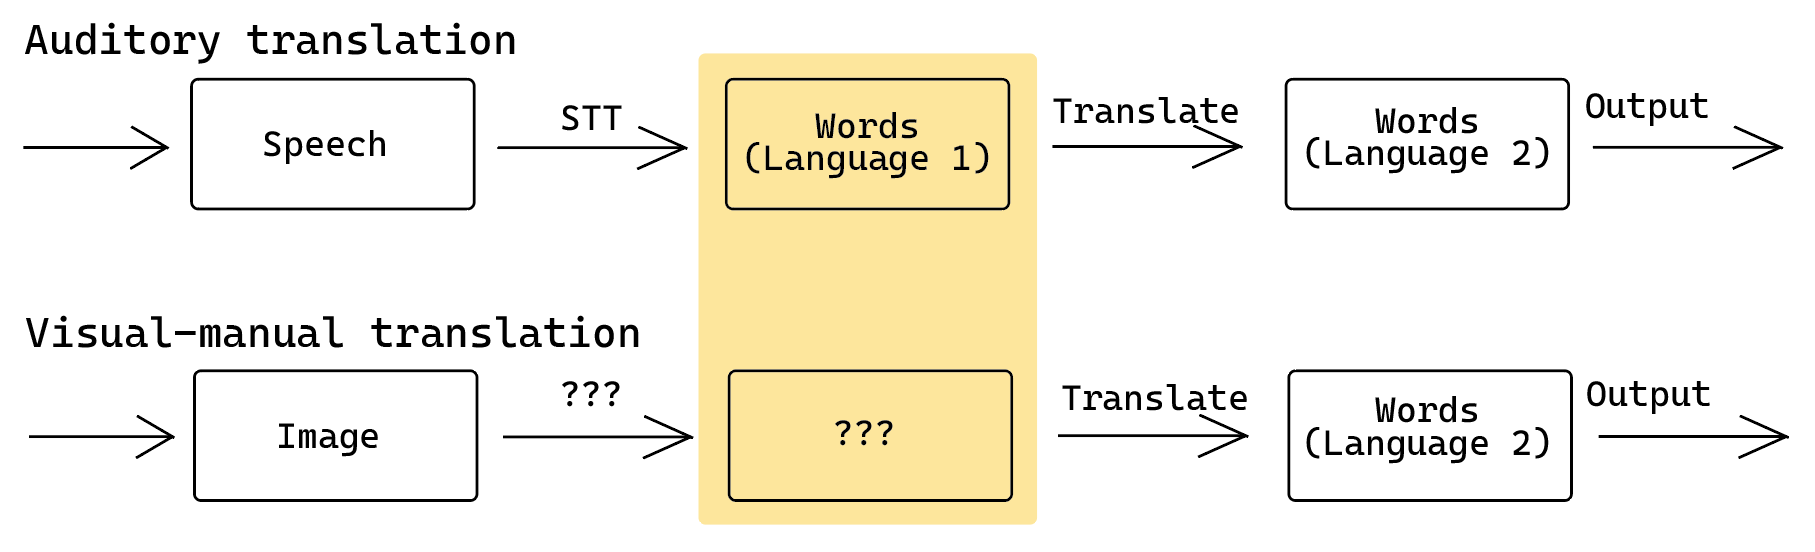
\includegraphics[width=13cm]{audVsVM.png}
        \\
        \raggedright \textit{
        Figure 1: Temporary diagram showcasing the pipeline of auditory language translation vs visual-manual language translation.
        }
    \end{center}

    This project aims to alleviate these challenges by designing and developing an scalable visual-manual interface using a multitude of approaches. This report will document the problem solving, design, development, and analysis of a program designed to overcome the challenges of said interface for signed language interpretation.


\section{Pre-requisites Knowledges}
    This section will provide most of the technical prerequisite knowledge to understanding the approaches to the design on the program and the implementation of the program itself. This section will only include a very brief and high level explanation of the concepts at hand.

    \subsection{American Sign Language}
        There are approximately 70 million deaf people worldwide, who collectively use over 300 signed languages. Amongst those communities, the American Sign Language (ASL) is commonly accepted as a lingua franca (common language), with many deaf individuals learning ASL as a secondary language as a means to communicate with deaf people from different countries / communities. Over 500,000 people in the United States of America (USA) use ASL as their native language; this statistic does not even include non-native (second language) users of ASL or native users of ASL outside of the USA (such as Canada). These signed languages are vital to the enabling of social interactions within these communities. 

        \paraskip

        \noindent\textbf{Lack of Digital Support:} Even with such a large userbase, ASL (or any signed language for that matter) severly lacks digital language support. According a study conducted by ACL Anthology - ”Assessing Digital Language Support on a Global Scale”, ASL is on the ”Emerging” category. This means the language has some content in digital form (mainly videos on social media or educational platforms), but lacks programs for machine interpretation.

        \paraskip

        \noindent\textbf{Lack of Writing System:} Lastly, ASL (or most signed language for that matter) does not have a common writing system. There have been attempts to develop a written interface for ASL, such as ASLWrite, but unfortunately has not been widely adapted by the deaf community.

        \paraskip

        \noindent\textbf{Phonological Parameters:} ASL, like most other sign languages, have parameter other than hand shape to form words. These are known as phonological parameters; these include factors such as hand movement, referential locations, facial expression, etc. This makes developing a digital ASL translator a highly complicated problem. 


    \subsection{Deep Learning Approach (ConvNet)}
        Convolutional Neural Networks (AKA ConvNets or CNNs) are a type of deep learning neural network that specialises in image processing tasks. The main difference between ConvNets and a vanilla neural networks is the ConvNet's ability to maintain spacial relations and dimentional information. This is due to the ConvNet not flattening the data before feature extraction. ConvNets are built with many different types of layers - convolution layers (feature extraction), pooling layers (compression) and ReLU layers (activation function).

        \paraskip

        \noindent\textbf{Convolutional Layers: } Convolution layers feedforward using specialised weights known as kernels (or filters). Kernels are a matrix used for feature extraction, they work by sweeping over a map and applies an operation (typically dot product) over the window of which the kernels cover, the value extracted will be how likely that specific feature has been extracted. An example of this would be a single feature extraction layer of a ConvNet specifically designed for edge detection: 

        \begin{center}
            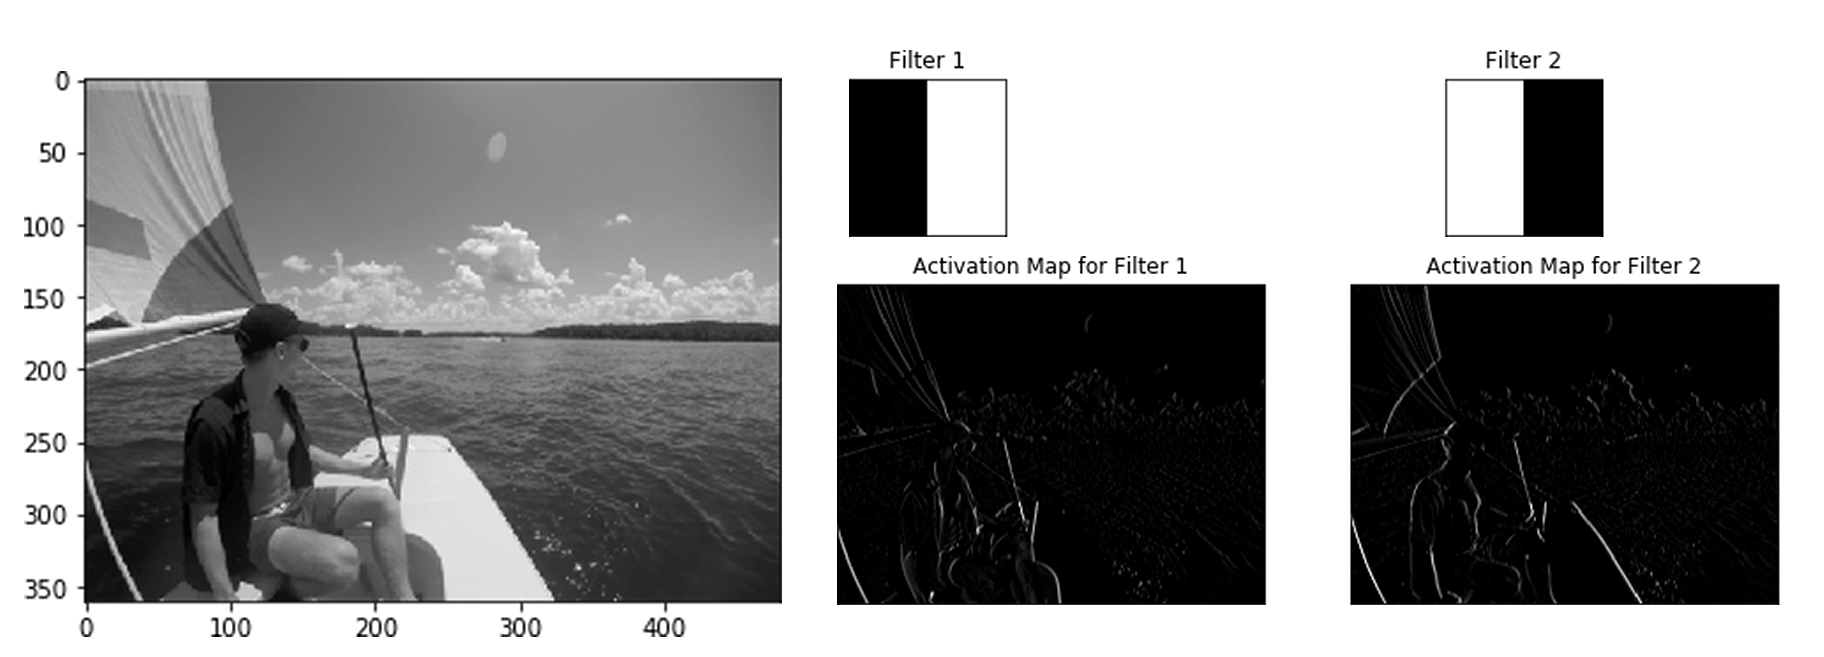
\includegraphics[width=12cm]{kernels.png}
            \\
            \raggedright \textit{
            Figure 1: Visualisation of Feature Maps Extracted from Preset Kernels for Edge Detection \cite{cnn goat}.
            }
        \end{center}
        
        \noindent This is but a high level explanation; in reality, the kernels are not manually crafted but generated using backpropagation during training with multiple layers of feature extraction.

        \paraskip
        \noindent\textbf{Pooling Layers: } Pooling layers feedforward a feature map compressed with a lossy compression designed to reduce the sizes of feature maps. This process drastically improves the speed of the neural network, however at the cost of negligable accuracy. Pooling layers sweep a window over the feature map not unlike the convolution layers; however, instead of applying an operation between a kernel and the window, it `pools' the values of the windows and outputs a result. Max-pooling returns the largest value within a window, min-pooling returns the smallest value within a window, and average-pooling returns the mean of all the values within a window. Which pooling algorithm depending on what tasks are at hand. All 3 pooling methods add translational and shift invariance to the model to varying degrees. Some pooling methods are better at reducing feature loss in certain situation than others.

        \begin{center}
            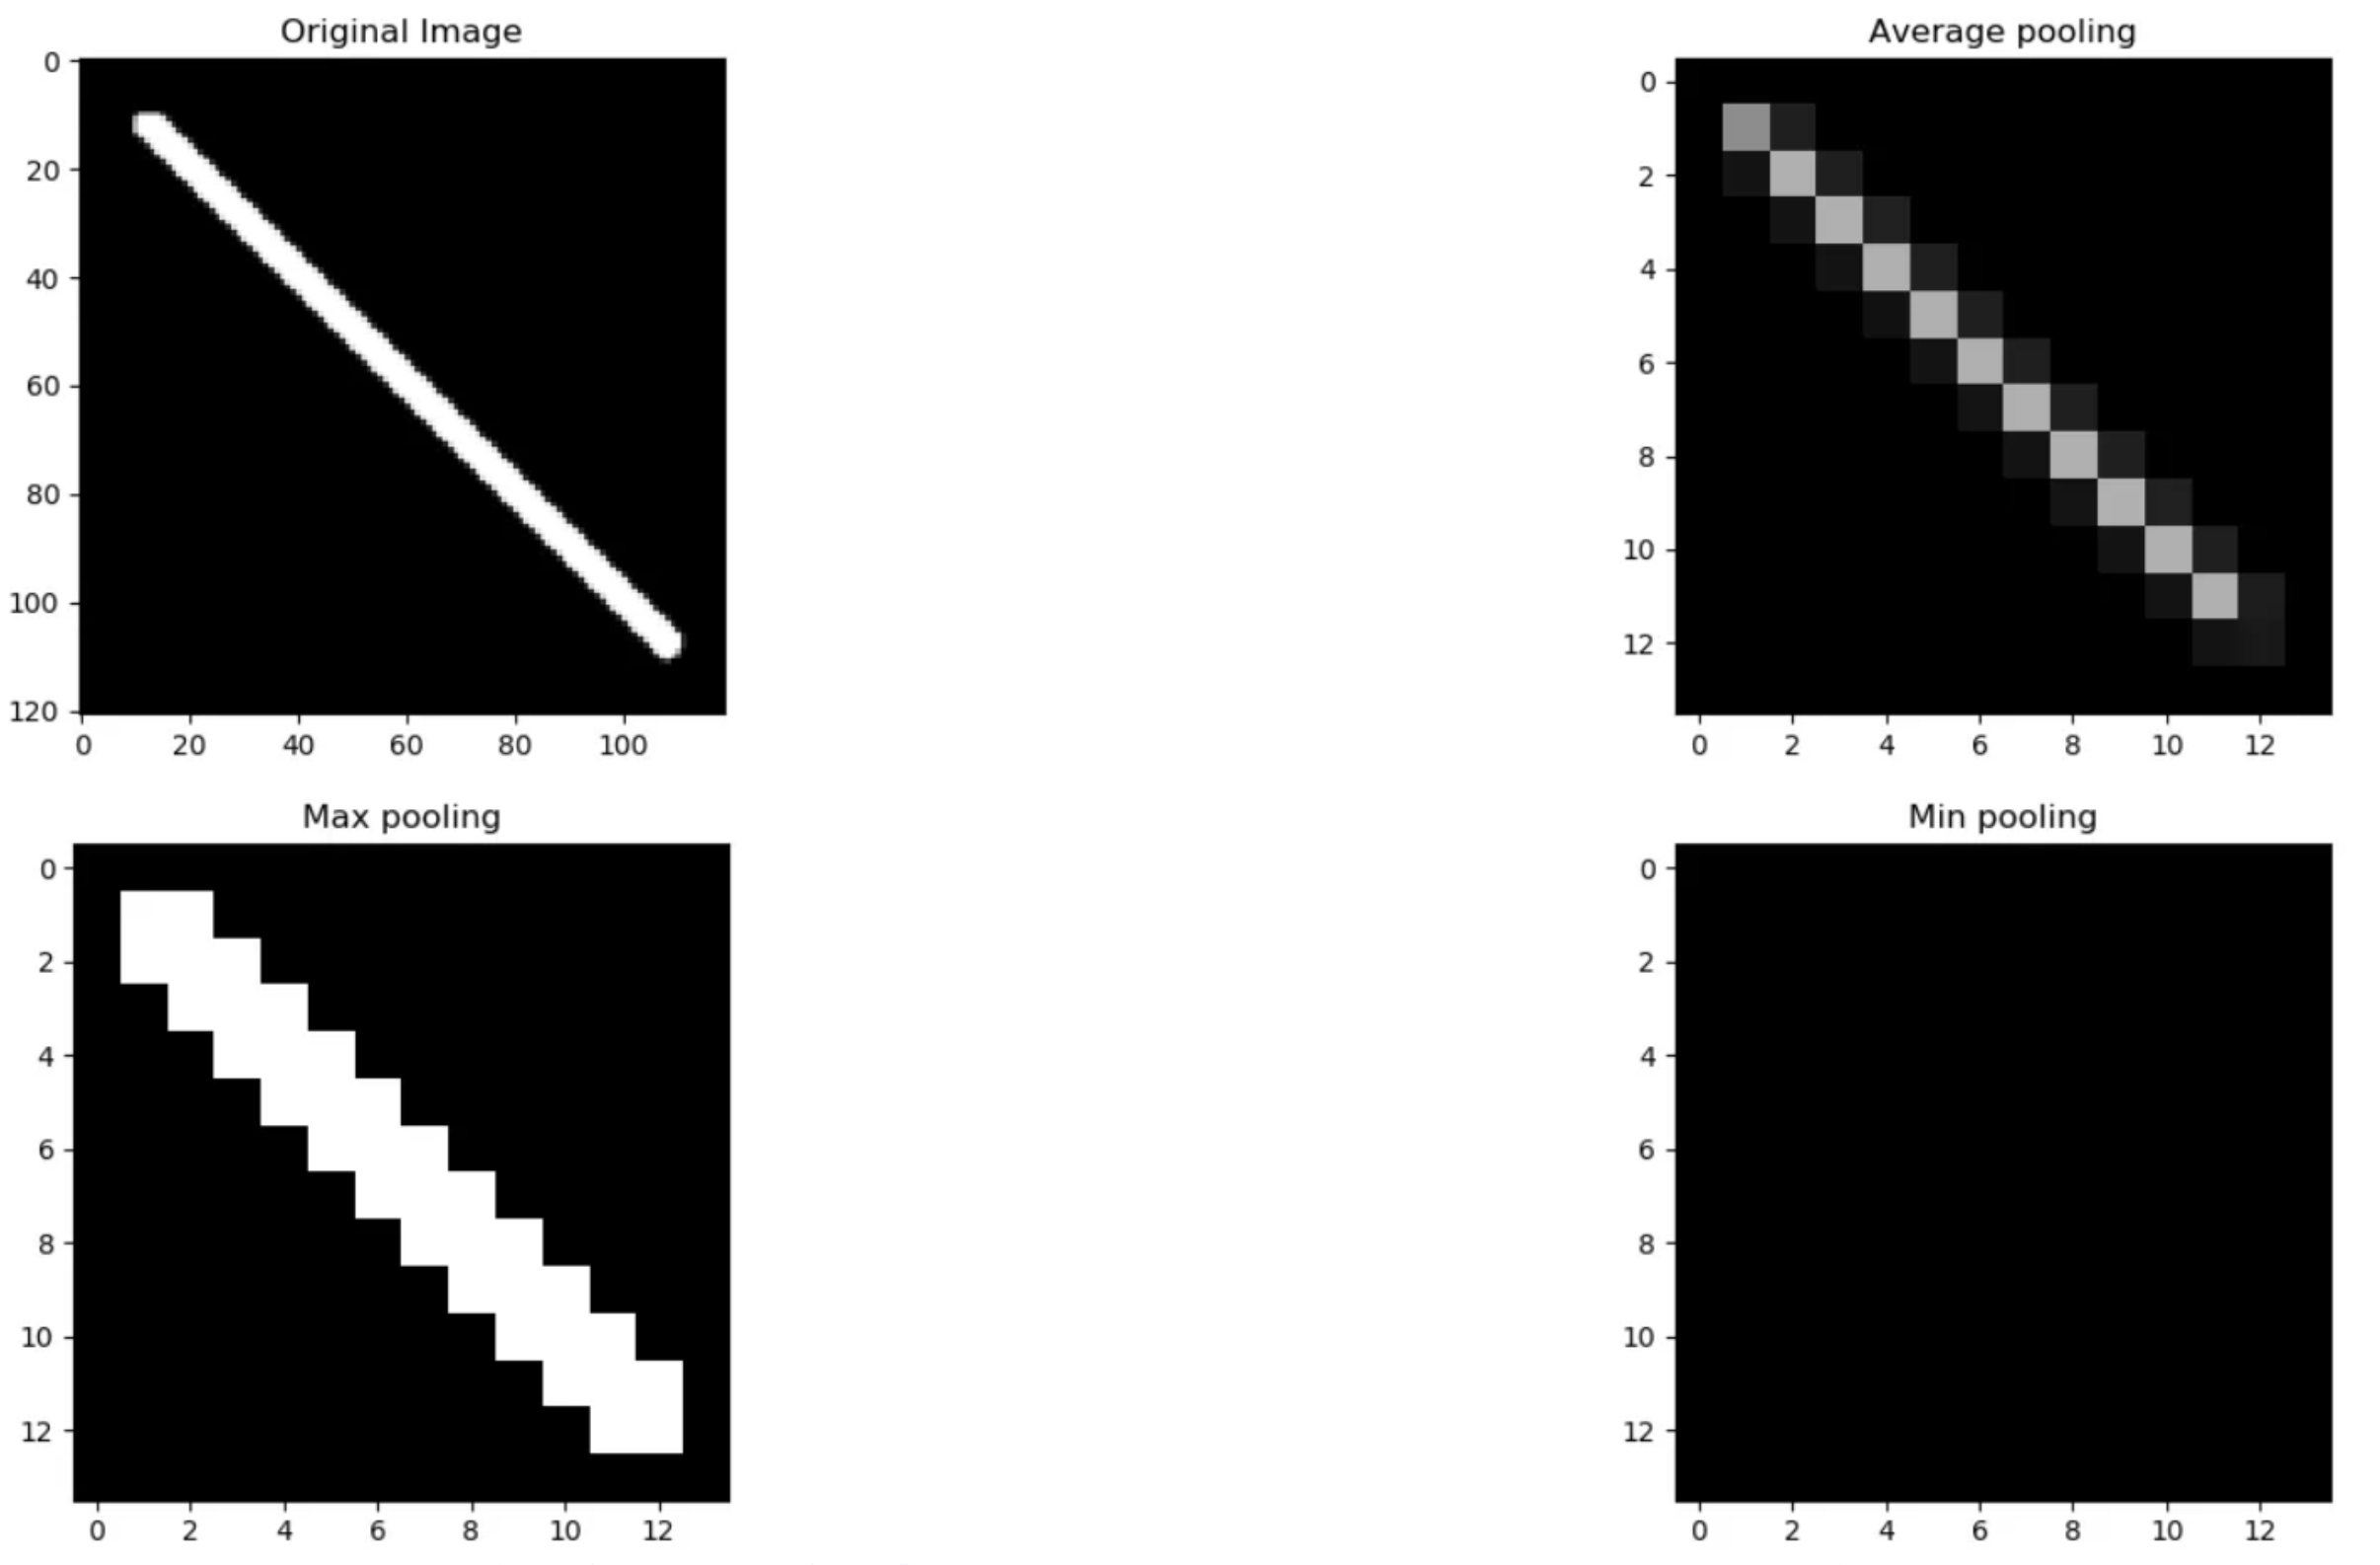
\includegraphics[width=6cm]{blackpool.png}
            \hspace{2cm}
            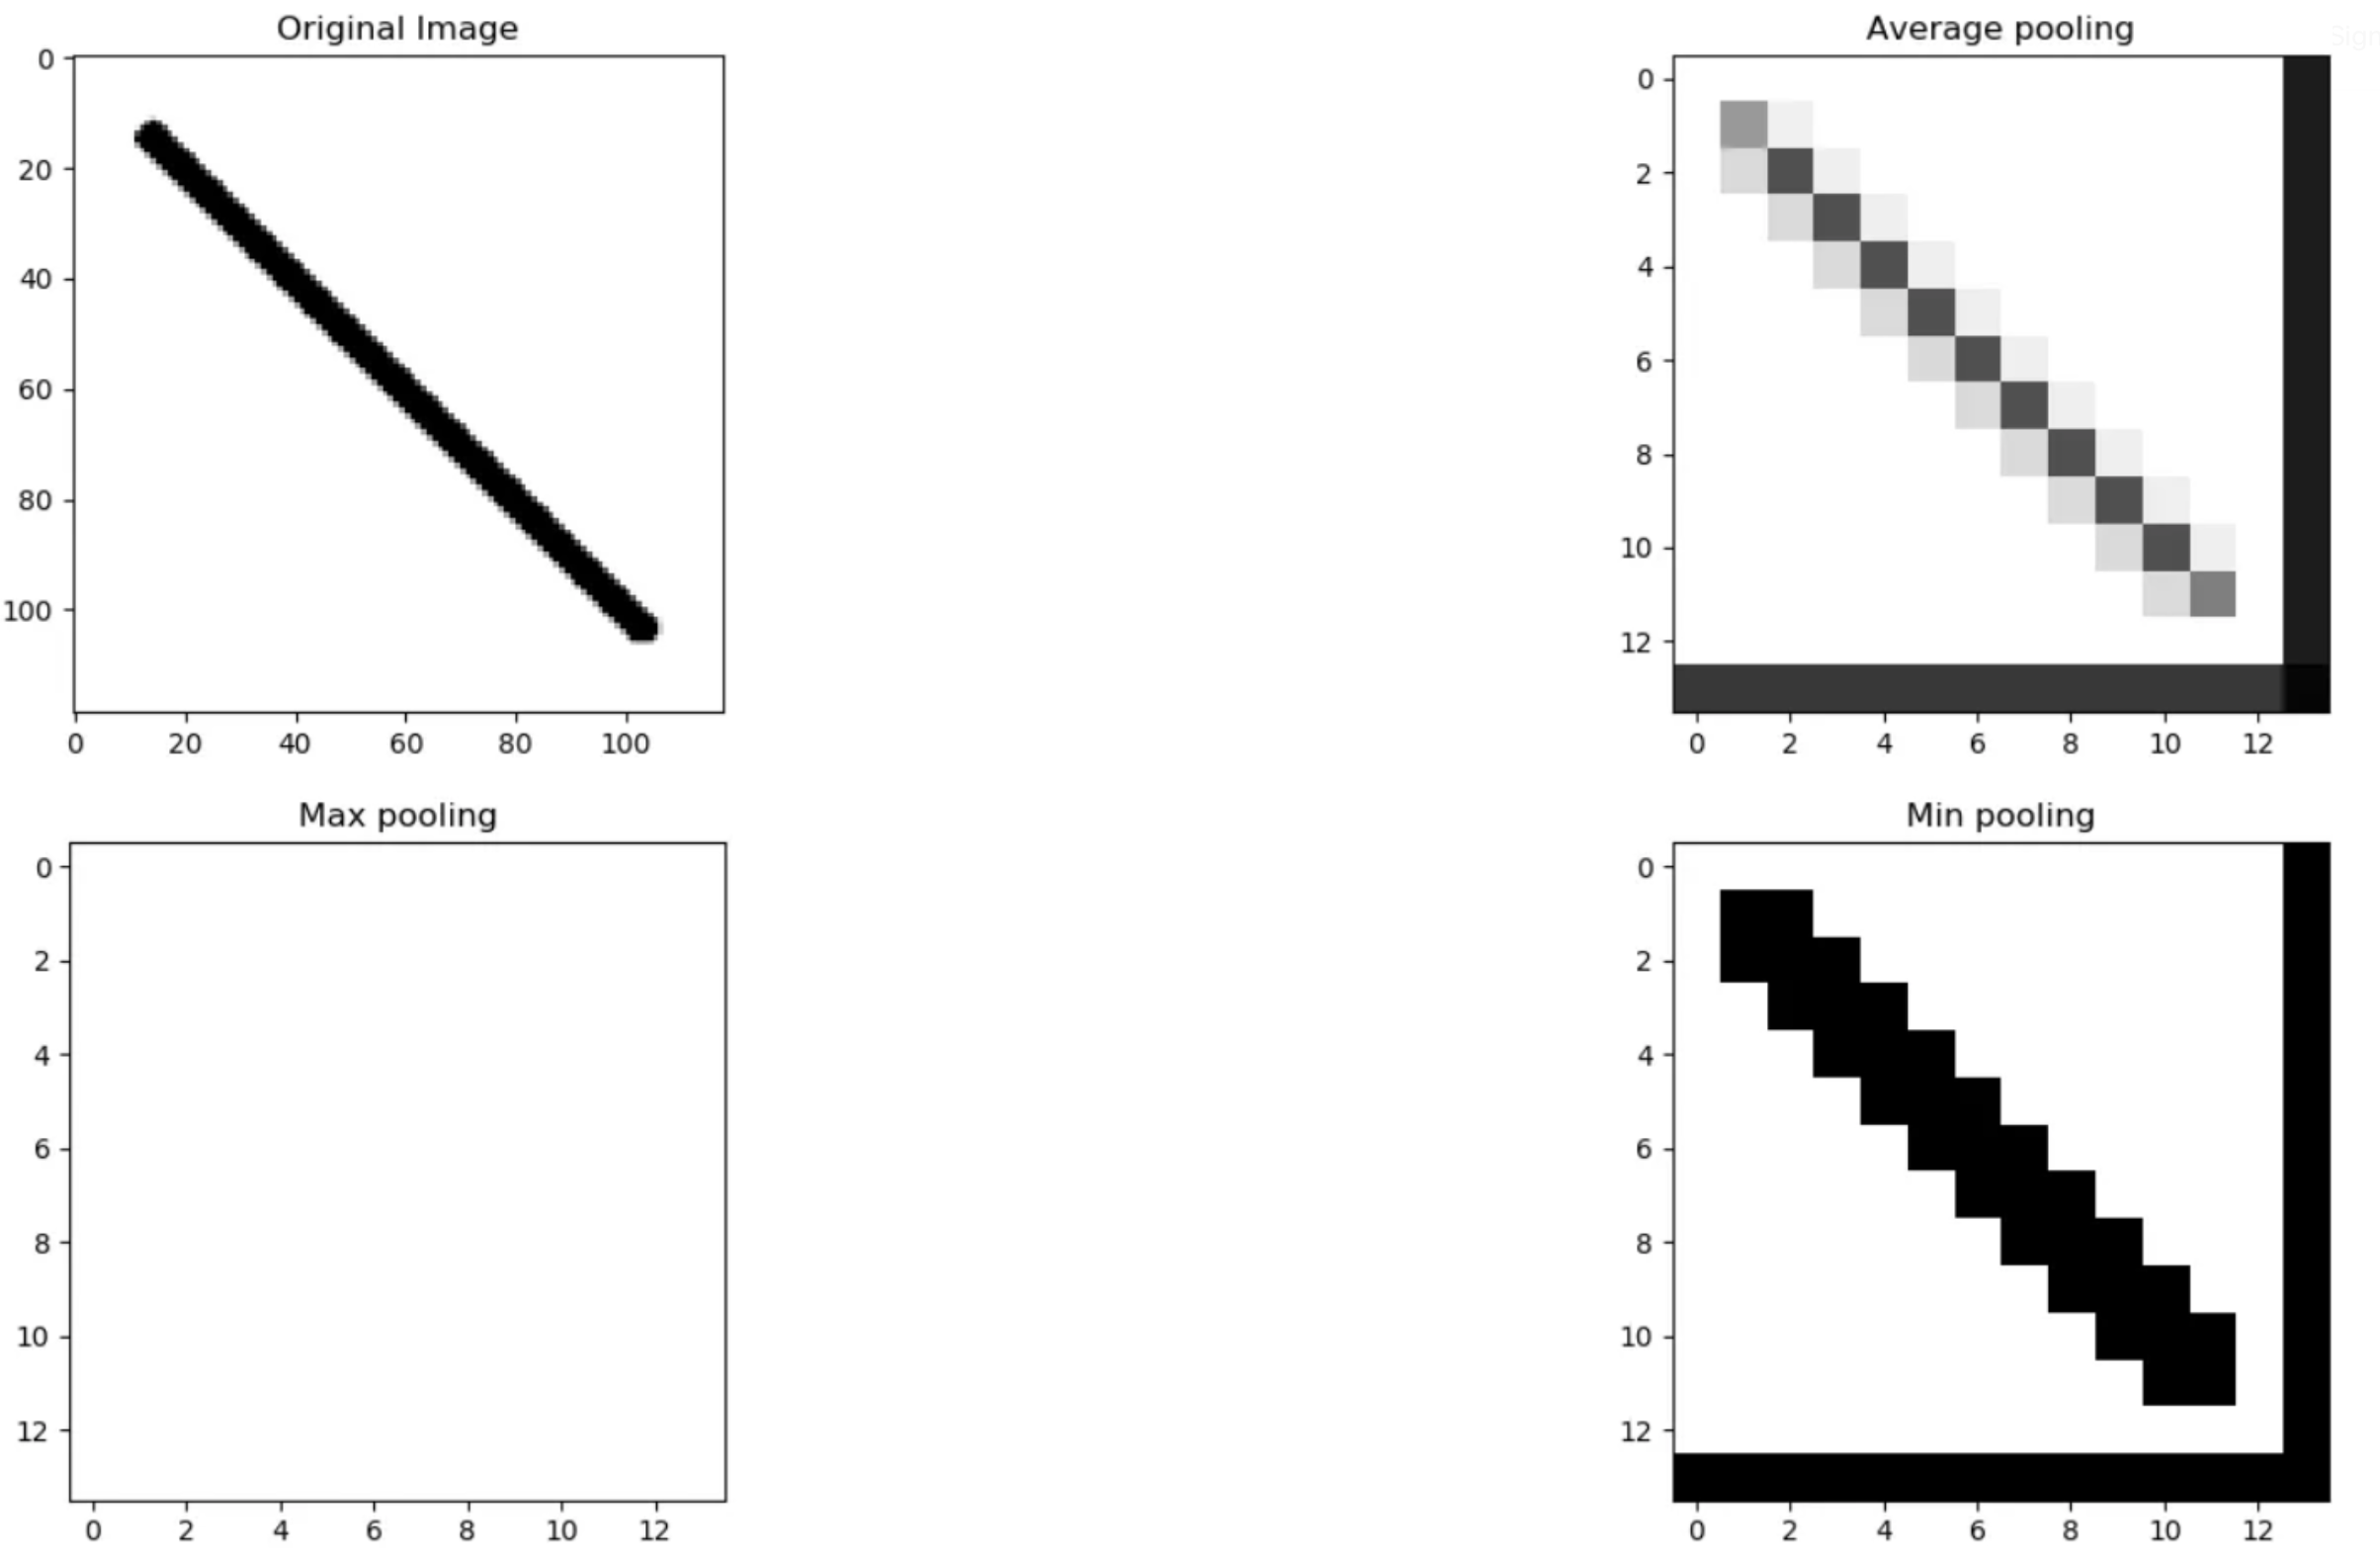
\includegraphics[width=6cm]{whitepool.png}
            \\
            \raggedright \textit{
            Figure 2: Pooling Effects on 2 Feature Maps (White Pixels Represent High Feature) \cite{poolingdiff}.
            }
        \end{center}

    \subsection{Hand Landmark Detection (OpenPose)}
        Hand landmark detection subset of pose estimatation specifically designed to identify joints of a hand. Due to the complex nature of the problem, deep learning solutions are often utilized for landmark detection. Pose estimatation is typically split into 2 distinct tasks - object awareness and joint extraction. This leads to 2 types of approaches to this problem - top-down and bottom-up. 
        
        \paraskip

        \noindent\textbf{Top-down vs Bottom-up: } Top-down is straight forward, it first detect the object in an image and then feature extract the joints from the object. Top-down approaches are excellent for multi-object pose estimation as it knows how many objects are in the scene and knows exactly what joints to expect within each object's bounding box. The problem with a top-down approach is that it is slow, it requires the intial image to be processed then every subsequent object detected within that image. Bottom-up does it in reverse, it first locates and detects all joints from an image, then reconstructs a object based on the joints. This results in an `only-look-once' effect allowing for significantly faster processing time. However, this approach struggles significantly with multiple objects, as different objects joints may be assigned to each other resulting in very inaccurate results. Top-down is a more accurate albeit slow method suitable for non time sensitive programs, while bottom-up is more suitable for real-time single object applications. 

        \paraskip
        \noindent\textbf{OpenPose's Architecture: } In 2019, Zhe Cao and his colleagues designed OpenPose - a framework that was designed as a multi-object bottom-up approach to pose-estimation. Cao et al, invented a technique they call the Parts-Affinity Field (PAF) to accurately assign joints to their respective objects, while maintaining the speedy `only look once' effect of a bottom-up solution. The PAF is a field built with a set of 2D vectors that represent the directions of the limbs between each sets of joints. Bipartite matching is then employed to assure no 2 same-typed joints connect to the same joint (E.g. 2 different top thumb joints cannot connect to the same bottom thumb joint).

        \vskip 0.2cm
        \begin{center}
            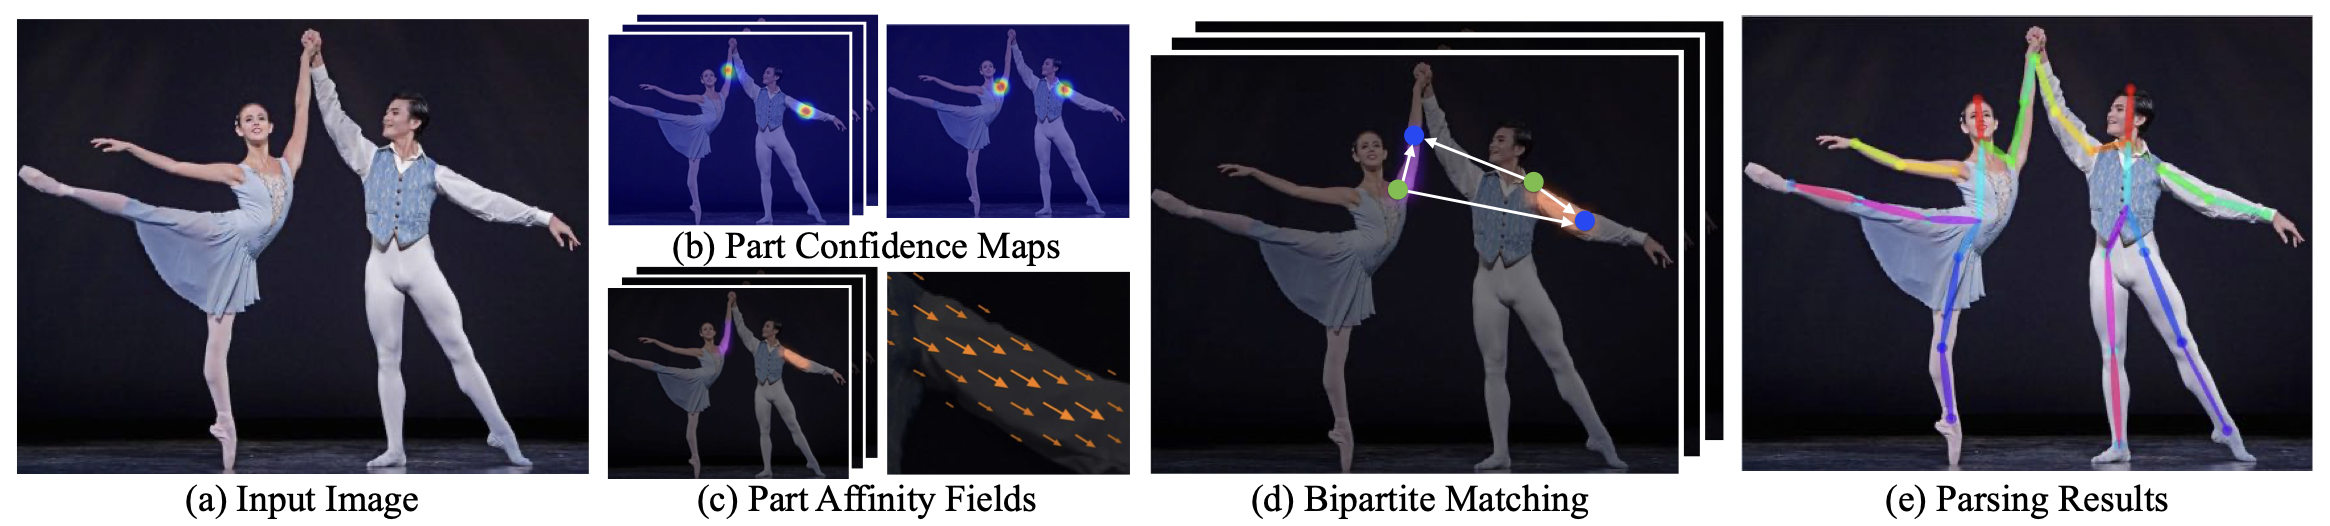
\includegraphics[width=14cm]{images/openpose.png}
            \\
            \raggedright \textit{
            Figure 3: Visualisation of the OpenPose Pipeline with PAF and Bipartite Matching.
            }
            \cite{openpose}
        \end{center}
        \vskip 0.2cm

        OpenPose also suggested a new way to train joint extractions (for any pose-estimation approaches) using a method called Multiview Bootstrapping. Essentially, difficult poses to estimate (or failed detections) are shot and then identified from multiple angles which make them easy to read. These poses are then reconstructed in a virtual 3D enviroment where, the now reconstructed pose, is projected into the failed detection and used to train the model to detect that specific difficult pose. This is an effective, albeit brutish, solution to limb occlusion (limbs covering joints) by teaching the model on specific poses where to `place' joints that go undetected.

        Even though OpenPose solves many of the problems with real-time pose estimation, there remains issues like object occlusion, motion blur and more. Fortunately, OpenPose is an open sourced model that allows new engineers to innovate and build upon what they have invented.


\section{Project Specification}
    This section will provide the project's goals and motivation, a high-level architecture of the program(s), a breakdown of requirements, and an evaluation method.

    \subsection{Project Goals and Motivation}
        Even though we have such a large deaf or hard of hearing population around the world, the lack of digitized support for these people is disheartening to say the least. This project strives to design an architecture for a sign language interpreter using both existing technologies and techniques invented specifically for this project. This project is also a comparative study between the custom visual-manual interface developed in this project (OpenHandmark) vs a traditional image classifier approach.
    
    \subsection{Project Overview (ASL Interpreter)}
        This subsection will contain a high-level design of a working visual-manual interface. This interface can be used for many purpose; for this project, the goal is a proof-of-concept sign language interpreter with scalable phonological parameters. The sign language used for this project will be ASL, due to its popular nature and the ease of access for its learning resources. 

        \paraskip

        \noindent\textbf{Static Symbol Classifier: } A static symbol classifier is the basis of a visual-manual interpreters. This approach first takes in an image as input, then uses a ConvNet or similar neural networks to classify the image based on what symbol the hand is making. Although this model may be very easy to develop, its accuracy is heavy swayed and affected by background change, finger occlusion and training data inconsistancies. Hand landmarking technology alleviates these problems by extracting joint and limb features then using those explicit features to classify into a symbol. This diagram illustrates this model:

        \begin{center}
            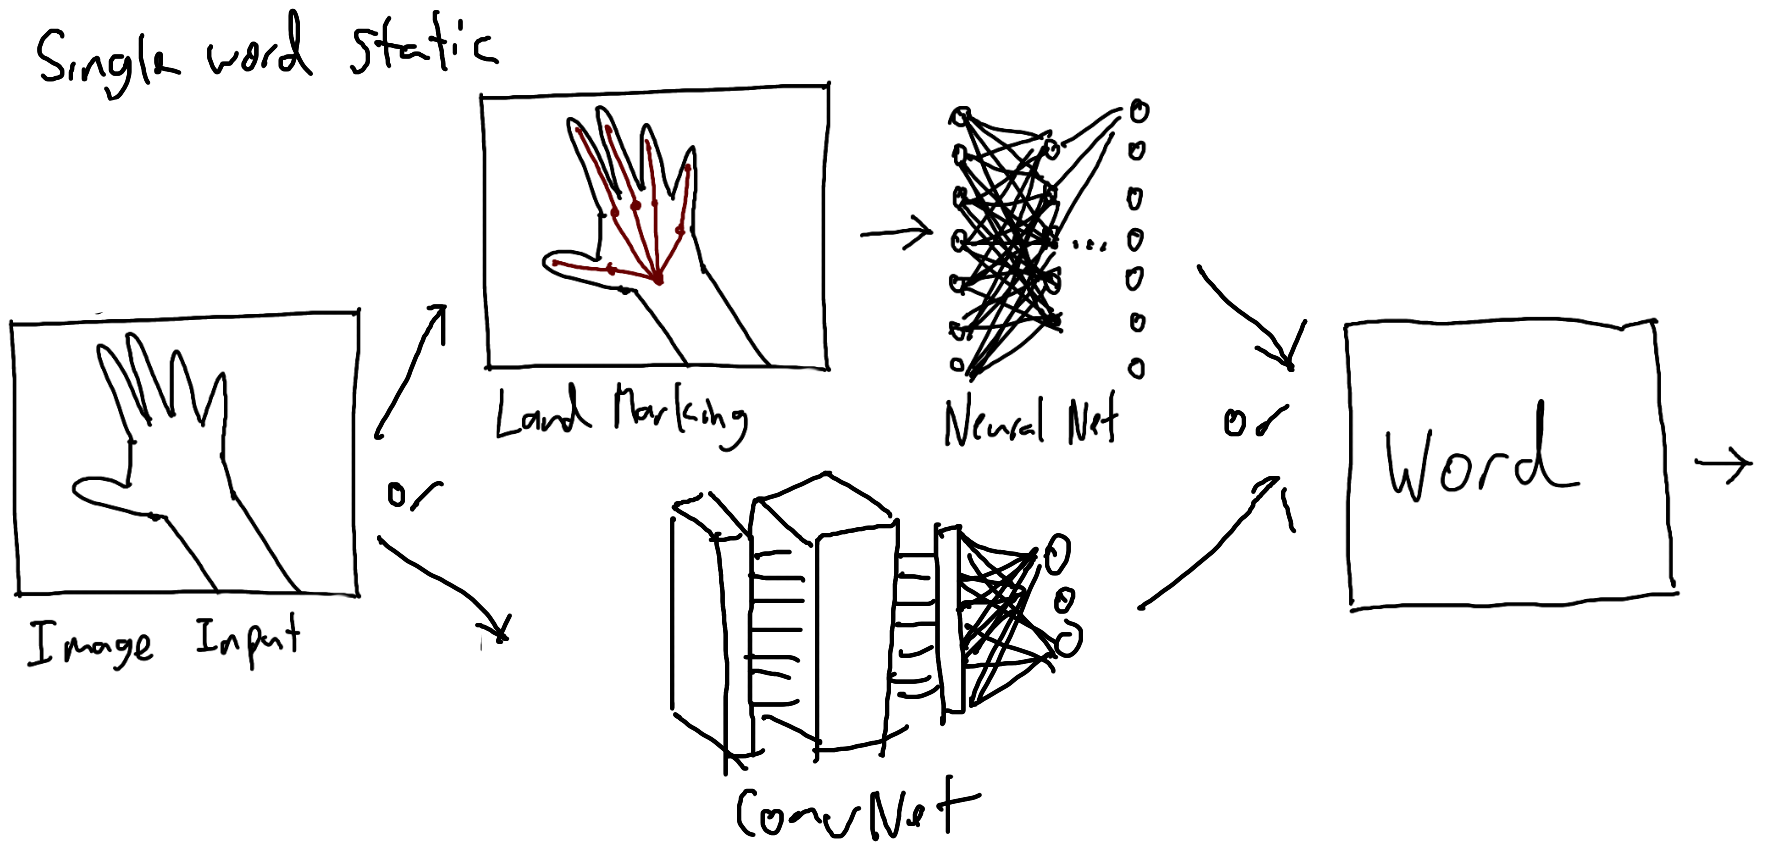
\includegraphics[width=12cm]{images/staticModel.png}
            \\
            \raggedright \textit{
            Figure 4: Visualisation of the Pipeline for Static Image Interpreter
            }
        \end{center}

        The problem with the model above is its incapability to read other phonological parameter, therefore we need to alter the pipeline. 
        
        \paraskip

        \noindent\textbf{Landmarking Approach: } Utilizing hand landmarking technology, we can determine the position of the hand and its respective joints within each individual frame. This stream of coordinates can be used to for many things, such as, calculate the direction(s) of the hands motion using displacement vectors. This group of coordinates can even be used for classifying the symbols themselves.

        \paraskip

        \noindent\textbf{Scaling with Phonological Parameters: } With the symbols extracted and the motion of the hands detected, these can now be grouped together to form a digitally comprehensible written representation. To better understand this, let's use the example of the ASL word - `hello'. `Hello' is formed by an open palm (same sign as the letter B), in a left to right motion; the same way you would typically wave. The model will detect through multiple static frame the letter B, then it will detect the motion of the hand based on how the coordinates of the palm is displaced. The model will then output the information formatted like so, `$A \leftarrow \rightarrow$'.

        \begin{center}
            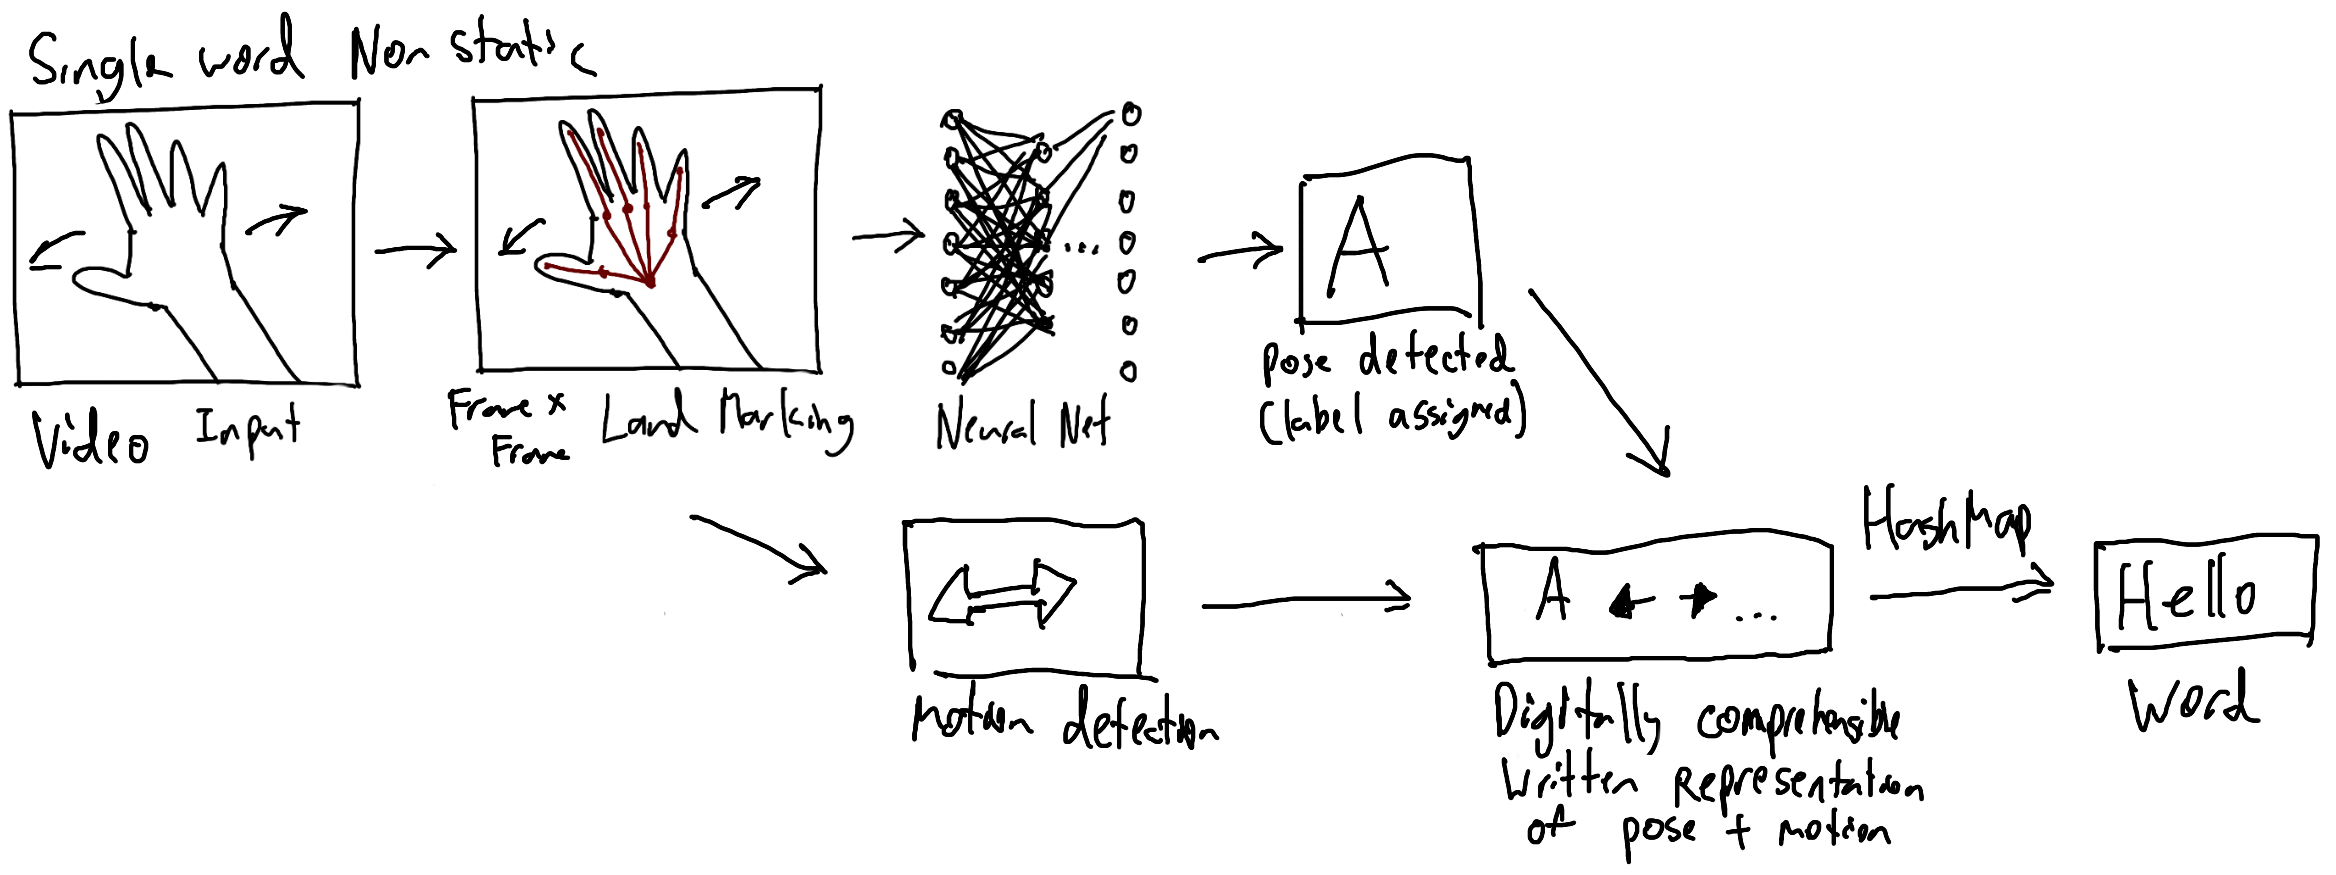
\includegraphics[width=12cm]{images/nonstaticModel.png}
            \\
            \raggedright \textit{
            Figure 5: Visualisation of the Pipeline for Dynamic Image Interpreter
            }
        \end{center}
        
        This solution of having a written medium with extracted features represented as respective characters can be scaled to any phonological parameters, granted they can be digitally representable. Due to time constraints, and as this is only a proof-of-concept, the program will only include 2 of the most important phonological parameter - hand pose and hand movement.

        \paraskip

        \noindent\textbf{Symbol Condensation: }
        A problem we encounter is how predictions and results from multiple symbols can interact with each other to form a word. This problem arises from the model having no idea when to seperate a symbol from another. Assuming the model runs inferences on 12 frames per second, if every frame's prediction is considered, the output will be 12 symbols. This is a problem as a single hand pose could be held for longer than $1/12_{th}$ of a second. An algorithm will have to be designed to condense these outputs. A simple solution would be to simply condense all repeating symbols into a single one (e.g. AAABBAAA -> ABA); however, this solution would only work granted a near $100\%$ accuracy rate as any prediction error over a held pose will cause inaccuracy flickers (e.g. AAASAASAA -> ASASA which is unintended). 
        
        Therefore, a custom 2-step algorithm leveraging temporal information can be used to stablize inaccuracies and condense symbols overall. Over a video or stream, each frame's symbol prediction will be appended to a first-in-first-out queue. We assign a buffer value which will be the queue's length, whenever the queue is full (when the next frame is processed), the first prediction inserted will be popped. On any given frame, the current true prediction will be most common element in the queue. This will eliminate the problem of requiring $100\%$ accuracy to use the simple condensing solution suggested above. The simple condensing algorithm proposed in the paragraph above is then applied to the true prediction stream, giving us a successful segmented sentence.This algorithm can solve this symbol segmentation issue, even over inaccuracy flickers. 

        \begin{center}
            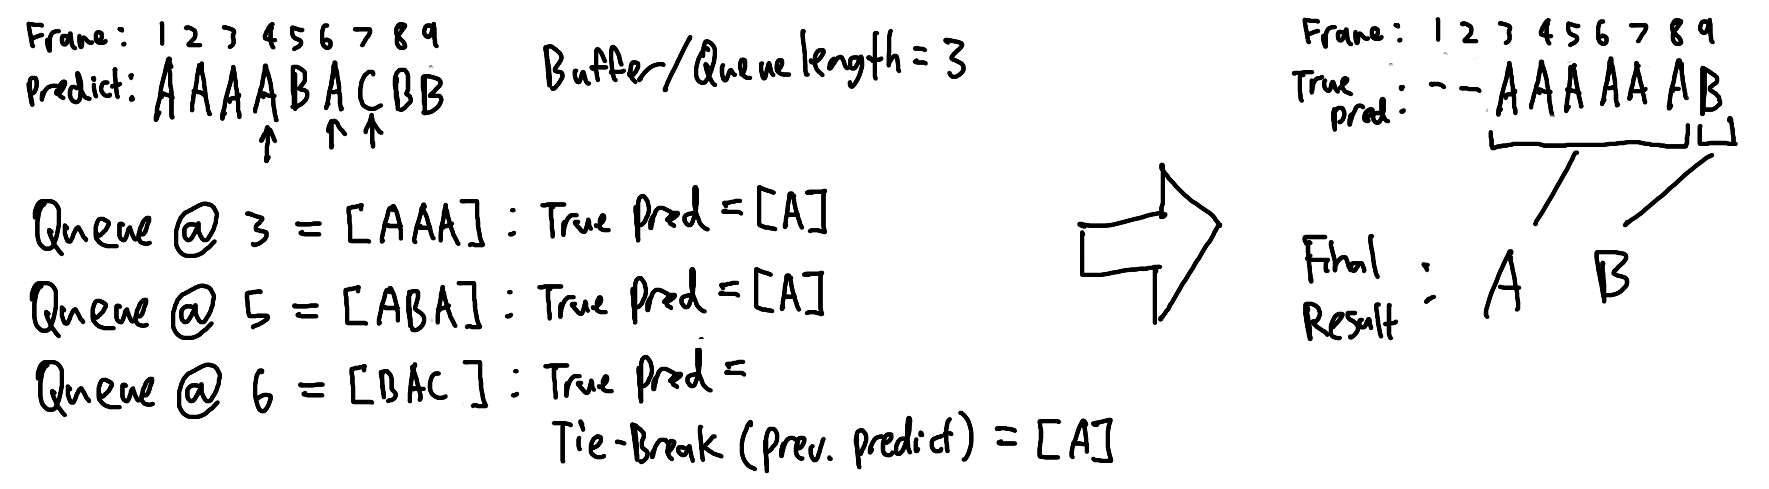
\includegraphics[width=12cm]{images/predOverTime.png}
            \\
            \raggedright \textit{
            Figure 6: Prediction Over Time Algorithm Visualised
            }
        \end{center}


    \subsection{Ethical and Societal Considerations}
        Due to the fact that I am not deaf or fluent in ASL, I do not have complete insight and understanding of the full nuances of the language, nor am I a part of the deaf community in discussion. To prevent myself from inappropriately representing the language, this project will only be a \textbf{proof-of-concept} utilizing a select few words and letters from the dictionary of ASL. The idea behind a digital ASL medium is also just a concept used for scaling the model to ASL's complex parameters beyond movement and posture. I am in no way trying to culturally appropriate the subject at hand; this study, if proved to be useful, should be pursued further alongside an ASL expert or members of the deaf community.

    \subsection{Project Tasks}
        A breakdown of the tasks at hand.

        \begin{center}
        \begin{tabularx}{1\textwidth}
            { 
            | >{\raggedright\arraybackslash\hsize=.25\hsize}X 
            | >{\raggedright\arraybackslash\hsize=.75\hsize}X | 
            }
            \hline
                \textbf{Task} & \textbf{Task Description} \\ [0.5ex] 
            \hline

            \hline
            \hline
                \multicolumn{2}{| l |}{\textit{ConvNet Approach}} \\ [0.2cm]
                \hline
                Data Preprocessing & Readying the training and validation datasets to be in a standard readable format for both programs. \\ [0.7cm]
                \hline
                Implement a ConvNet Image Classifier & Implement an image classifier using a ConvNet architecture. \\ [0.7cm]
                \hline
                Train Classifier & Train the ConvNet. \\ [0.7cm]
                \hline
                Symbol Condenser & Uses the custom 2-step algorithm designed above to stablize and condense symbol predictions. \\ [0.7cm]
                \hline
                Implement Real-Time Demo & Implement a real-time demo using OpenCV to process and classify images coming from a stream. \\ [0.7cm]
            \hline
            
            \hline
            \hline
                \multicolumn{2}{| l |}{\textit{OpenHandmark's Approach}} \\ [0.2cm]
                \hline
                Implement Hand Landmarker & Implement the hand pose estimation program with MediaPipe or OpenPose.\\ [0.7cm]
                \hline
                Landmark Normalizer & Automate the normalisation of the output data. \\ [0.7cm]
                \hline 
                Data Preprocessing & Running the dataset through the landmarker and normalizer, annotating every hand and its joints. \\ [0.7cm]
                \hline
                Implement Landmark Classifier Model & Implement a neural network for the post-processed dataset to recognise ASL alphabet. \\ [0.7cm]
                \hline 
                Train Landmark Classifier Model & Train the classifier on the post-processed dataset to recognise ASL alphabet. \\ [0.7cm]
                \hline
                Motion Tracker & Module to determine the motions of the hand throughout a video or stream. \\ [0.7cm]
                \hline
                Word Formation Algorithm & Uses the symbol condenser and other methods to form words based on motion and symbol segmentation. \\ [0.7cm]
                \hline
                Sign Language Translator & Implements an typing interface that allows complex ASL words (containing at least 2 phonological parameters) to be translated. \\ [0.7cm]
            \hline
        \end{tabularx}
        \end{center}

\section{Program Design}
    \subsection{Design Iterations}
        Before the final iteration of the program can be explored, the first few iterations of the model must also be explored to emphasize the problems faced and the solutions found. During the initial phases, this project was only meant to be a static hand sign classifier; however, due to an increasing scope, this project now presents a custom dynamic and real-time visual-manual interface. For this paper, the developmental details of the progression between the first model (image classifier approach) to the final one (landmark assisted approach) will be reported. This includes the inner workings of the models, its problems and the evolutions required to solve them. A simple explanation of each model will be presented in this subsection.

        \paraskip

        \noindent\textbf{ConvNet Approach: } The first model was a static image recognition approach using InceptionNet V1 (AKA GoogLeNet) to classify each hand's pose. This approach has significant limitations due to its slow inference and training times. The first major limitation of this model is the fact that it is susceptible to background changes and ambient lighting, resulting in a very low accuracy outside of the settings of the training dataset. There are also other limitations of this model such as its complete inability to scale to other phonological parameters.

        \paraskip

        \noindent\textbf{Landmark Assisted Approach: } This is the definitive model of the project, aimed to completely eliminate the background and lighting problem by explicitly feature extracting hand landmarks. This allows the features to be directly classified using a significantly more lightweight neural network via a vanilla multi-layered perceptron (MLP). This also drastically increase the scalability, as the first part of the model (hand landmarking) will be in constant time. The hand landmarks also provides a clear metric for where the hands are in regards to the image, allowing us to modify the model to include phonological parameters in regards to referential locations and movements.

    \subsection{Program Architecture (ConvNet Approach)}
        Convolutional neural networks are used for the first interation of the visual-manual interface. This will be commonly referred to as the \textbf{static model}, due to its limitations to only classify words from a static frame. The idea behind the use of ConvNets is due to the fact that they are excellent at classifying data representable in image form. This allows us to implement a ConvNet and simply feed in the data raw for training. 
        
        \paraskip

        \noindent\textbf{Why GoogLeNet: } For this iteration's model, GoogLeNet (or InceptionNet v1) was chosen due to it's resistance to differing saliency. Saliency is `the property by which an object stands out', in our case, the hand. This resistancy is required due to the fact that the hand will not always be within the same distance of the camera, sometimes taking more space within and the screen and sometimes taking less. Observe the following example:

        \begin{center}
            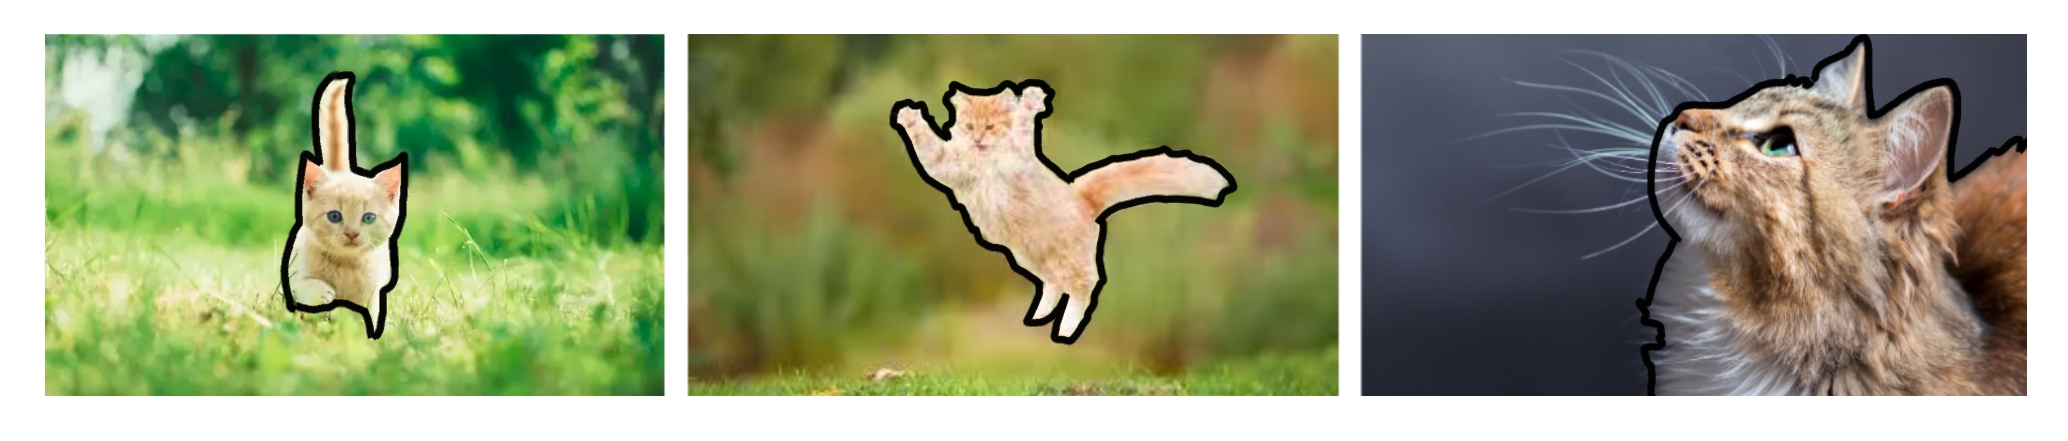
\includegraphics[width=15cm]{images/cats.png}
            \\
            \raggedright \textit{
            Figure 7: The areas the cats displace in the images are vastly different (outlined in black). Left takes up less space, right takes up more.
            }
        \end{center}

        The premise of GoogLeNet's architecture is based on solving 3 main problems - Specificity of kernel sizes, deep networks overfitting, and computationally expensive convolutional layers. Firstly, choosing the kernel sizes used to be highly limited to specific tasks. This is due to the fact that there is often a large variation between location and size of an object within an image; a large kernels are often used for objects distributed more globally, while smaller kernels are used objects distributed more locally. Secondly, deep neural networks are more prone to overfitting. This means a deep network will be familiar with data very similar with its training set and fails to have any level of accuracy with new data introduced from outside of the set. Lastly, convolutional layers are very computationally expensive. Stacking them naively will lead to very long processing times that don't necessarily translate to better accuracy.

        \paraskip

        \noindent\textbf{Inception Layers: } GoogLeNet solves these 3 problems by introducing a new type of convolutional layer called the `inception layer'. These inception layers allow for horizontal (instead of the traditional vertical) scaling, with kernels of differing size within the same level. Essentially the input feature map will be fed into multiple convolution and pooling layers of differing kernel sizes. The output of each of these operations will then be concantenated into one output map. This allows for increased flexibility for the network to learn stacks of features within the same level, solving our first problem. This also decreases the depth of the network as a whole by scaling its layers horizontally, overall decreasing overfit and giving a better accuracy per layer and per computer resources.

        \begin{center}
            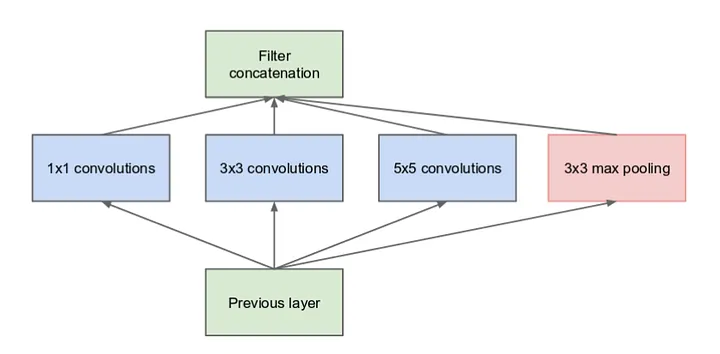
\includegraphics[width=12cm]{images/inceptionlayer.png}
            \\
            \raggedright \textit{
            Figure 8: Naive view of a single inception layer.
            }
        \end{center}

        \paraskip

        \noindent\textbf{Canny Edge Modification: } The next iteration directly proceeding the GoogLeNet approach is the idea to preprocess all image data with a canny edge function. A canny edge function finds contrasting pixel values in an image and uses them to infer where an edge is. This was done in an attempt to ease the low accuracy rates caused by background influences; however, more complex backgrounds will continue to influence the image. A max-pool layer will also have to be applied to downscale the image while retaining the white edges (see Figure 2). 

        \begin{center}
            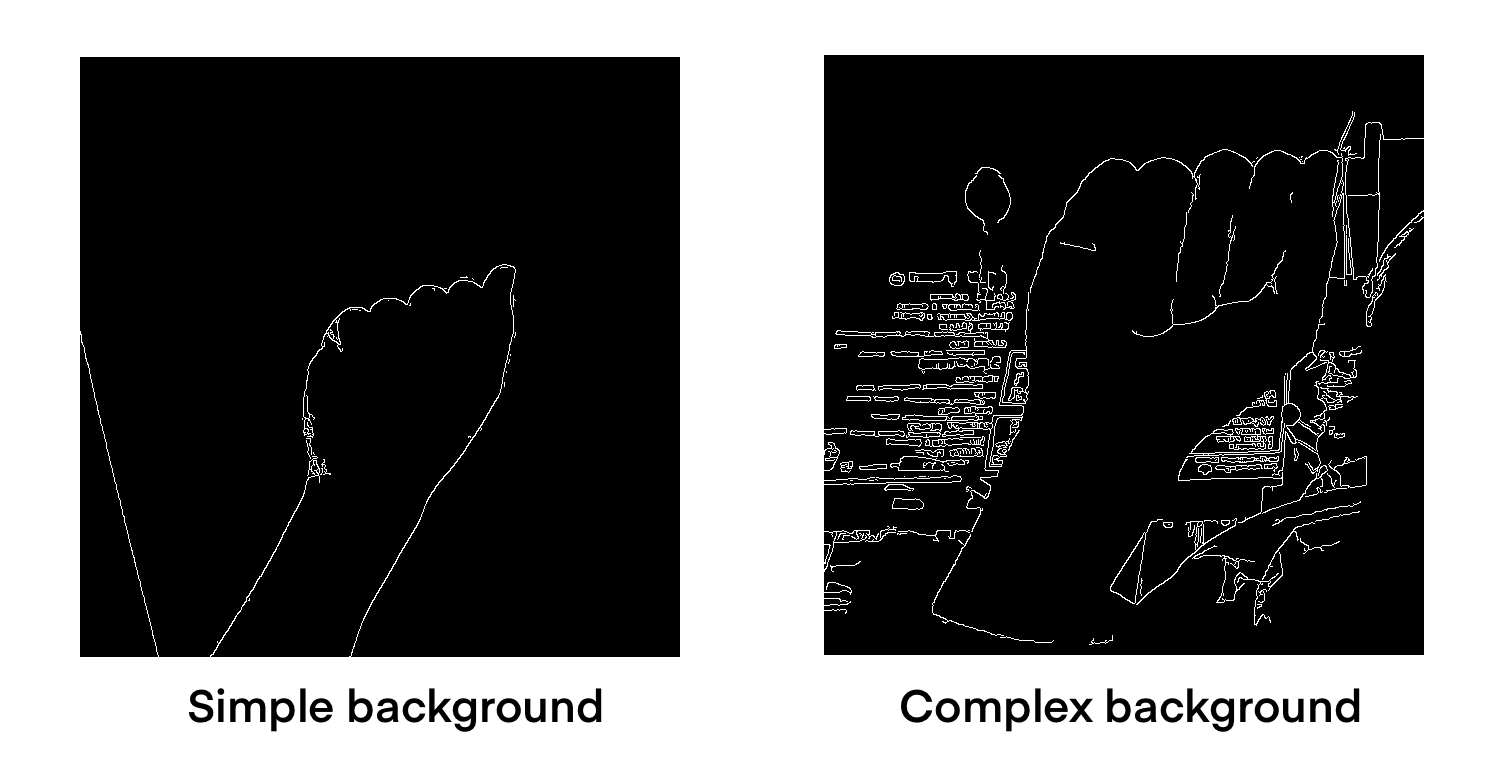
\includegraphics[width=10cm]{images/canny.png}
            \\
            \raggedright \textit{
            Figure 9: Visualisation of how canny edge can be used to alleviate background influence to a certain degree only.
            }
        \end{center}

    \subsection{Program Architecture (Hand Landmark Approach)}
        The final iteration of this project uses pose estimation technology to extract hand landmarks to be used for classification. This model will be referred to as the \textbf{dynamic model}, due to it's ability to read and parse movement and changes in positions and symbols through multiple frames. The main premise of this approach is due to the idea that vanilla MLPs are easier to train and have a significantly faster runtime than ConvNets. This increase in speed is leveraged in hopes to make the program viable for real-time processing. There are other benefits to using this explicit feature extraction method as well - Hand tracking, even more resistance to changes in saliency (through normalisation), and complete background immunity. Since the technology behind hand landmarking has been explained in a previous section (see section 2.3), this section will take a higher level explanation of the program architecture.

        \paraskip

        \noindent\textbf{Landmark Normalisation: } Each joint is scale and position normalized before feeding into the neural network for the sake of consistency. For position normalisation, we set the bottom of the palm at (0,0) and scale each joint accordingly by setting the original bottom palm landmark as the offset. Each joint will then have its coordinate values subtracted by the palm offsets. This allows the same hand pose to be wherever in the image and still return the same coordinate values. The scale normalisation is simply min-max scaling between all the coordinates. The x and y distances between each landmark will still be on the same ratio but bound between either a relative or arbitrary maximum and minimum value, typically set between 0 and 1; therefore, preserving the most important feature (the ratio between limbs) while gaining data consistency. Relative min-max scales the values between the largest and smallest values within the original table, squishing them between 1 and 0. Arbitrary min-max scales does essentially the same but forces the new largest and smallest value to be between an $a$ and $b$ value. This allows for the same hand pose to be as close or as far away from the camera and still return the same coordinate values. The equations for both min-max scaling is as follows:

        \vskip 0.3cm
        \[
        \text{\bf{Relative Min-Max: }} x^{'} = \frac{x-min(x)}{max(x)-min(x)} 
        \]

        \[
        \text{\bf{Arbitrary Min-Max: }} x^{'} = a + \frac{(x-min(x))*(b-a)}{max(x)-min(x)}
        \] 
        \vskip 0.3cm

        \paraskip

        \noindent\textbf{Location and Motion Tracking: } Hand tracking will allow us to start scaling towards other location and movement based phonological parameters. There are 2 ways to track the location of the hand within the image - average coordinates and palm coordinate. The average coordinate way of tracking will be to find the mean of all x-coordinates and mean of all y-coordinates as the total location of the hand. This method is good for when the a certain joint's prediction jitters and could be read by the program as wild movements. The palm coordinate method is simply represent the hands location by the bottom of the palm. It is a lot simpler to implement but also less accurate. The formula for average tracking is as follows:

        \[HandLocation = (\bar{HandX}, \bar{HandY}) \qquad{}
        \bar{HandX} = \frac{1}{n}\Sigma x_{joint} \qquad{}
        \bar{HandY}  = \frac{1}{n}\Sigma y_{joint}
        \]
        \vskip 0.3cm

        Movement can be tracked by calculating the difference between 2 consecutive frame's hand coordinate. The hand's overall coordinate can be obtained using the paragraphs above (either mean centered or palm centered). The difference in position between the overall hands position between 2 frames will be used to calculate the direction it is travelling at that instance. However, with this approach, even when the hand is as still as possible the camera will still detect micro-movements and translate that into a direction; therefore, we need an arbitrary threshold for how big a movement has to be before it is considered a movement. The direction detection will only classify an 8-way movement for this program - left, right, up, down and all the diagonals. Every movement within a single held pose will be logged until the hand pose is changed, then the direction that composes more than 30\% of the whole log will be considered for the word. 


        \subsection{Symbol Translation Module}
        Translation from symbols detected using the models above need to still be translated into English words. On the static model, words will have to simply formed using a combination of letters also known as fingerspelling. On the dynamic model, movement will also be parsed and read alongside the symbol. The parsed movements (obtained via the method in the subsection above), will be concantenated at the end of the symbol. These concantenated string will simply be referred to as tokens. The translation process will take 2 parts - the autocorrect and the actual translation. 
        
        \paraskip

        \noindent\textbf{Levenshtein's Distance: } The autocorrection is needed due to small inaccuracies can ruin the entire prediction. Levenshtein distance is an algorithm used to calculate a score for how different a string is to another. Every operation is has a score assigned to it (e.g. substitution is $+1$, deletion and insertion is $+0.5$); the Levenshtein distance is the aggregate score of all edit needed to be made from one string to become another. To autocorrect we simply need to find the levenshtein distance between our token and the dictionary of potential strings, then the string will the smallest distance will replace the token. If the string matches the token the distance will be 0 and no replacements need to be made. The algorithm used to find Levenshtein distance will be a weighted variant specific to this project; there will be weighted substitutions to every direction symbol. The substitution cost for a direction $x$ units away will be $x$, that way the futher the directions need to be corrected, the higher the cost.

        \paraskip

        \noindent\textbf{Translation: } Translation will simply be the autocorrected word looked-up through a hashmap. This is the fastest way to do it due to the average $O(1)$ search time. The space complexity of $O(n)$ can somewhat be neglected due to modern hardware. The entire English language has around 200,000 words, and ASL has around 100,000 words. Because translation has to be a 1 to 1 mapping, we only need entries for around 100,000 words. Assuming each English word has 10 characters, and ASL tokens around 4, we would need 1,400,000 characters in memory for the dictionary. This only takes up 1.4 megabyte of memory, which justifies the use of a hashmap given the speed benefits.
        

\section{Implementation}
    \subsection{Frameworks}
    This subsection will detail all the frameworks used for the implementation for the rest of the project. The proceeding sections will assume this section has been read.

    \begin{center}
        \begin{tabularx}{1\textwidth}
            { 
            | >{\raggedright\arraybackslash\hsize=.2\hsize}X 
            | >{\raggedright\arraybackslash\hsize=.8\hsize}X | 
            }
            \hline
                \textbf{Frameworks} & \textbf{Frameworks Description} \\ [0.5ex] 
            \hline

            \hline
                \hline
                NumPy & Abbreviated from Numerical Python, it is an open-sourced library for fast math operations built with precompiled C code. Mainly used for the quick matrix manipulations and processings. \\
                \hline
                Pandas & An open-source library used for data manipulation and analysis. Allows for the efficient creation and processing of CSV files from raw unformed data. \\
                \hline
                PyTorch & Developed by Facebook's Research Lab as an open-sourced deep learning framework to easily implement custom AI models. Also allows for easy GPU training through CUDA cores on Nvidia cards or ANE on Apple devices.\\
                \hline
                OpenCV & An open-sourced computer vision library highly optimised for real-time applications. Allows for images to be altered and read en-mass and allows for frame by frame processing on videos or streams.\\
                \hline
                MediaPipe & Developed by Google and packaged with pretrained pose estimation weights and models. There is a \textbf{complete lack of documentation} (also no docstrings and poorly commented code) and requires a deep-dive into the source code to fully leverage the framework.\\
            \hline
        \end{tabularx}
        \end{center}

    \subsection{Static Interpreter (GoogLeNet)}
    This subsection will detail the overview of the implementation for the static visual-manual interpreter. This includes the data preprocessing, implementation of InceptionNet (AKA GoogLeNet), canny edge modifications, and any auxiliary modules. This will follow the monolithic structure shown in the diagram below:

    \begin{center}
        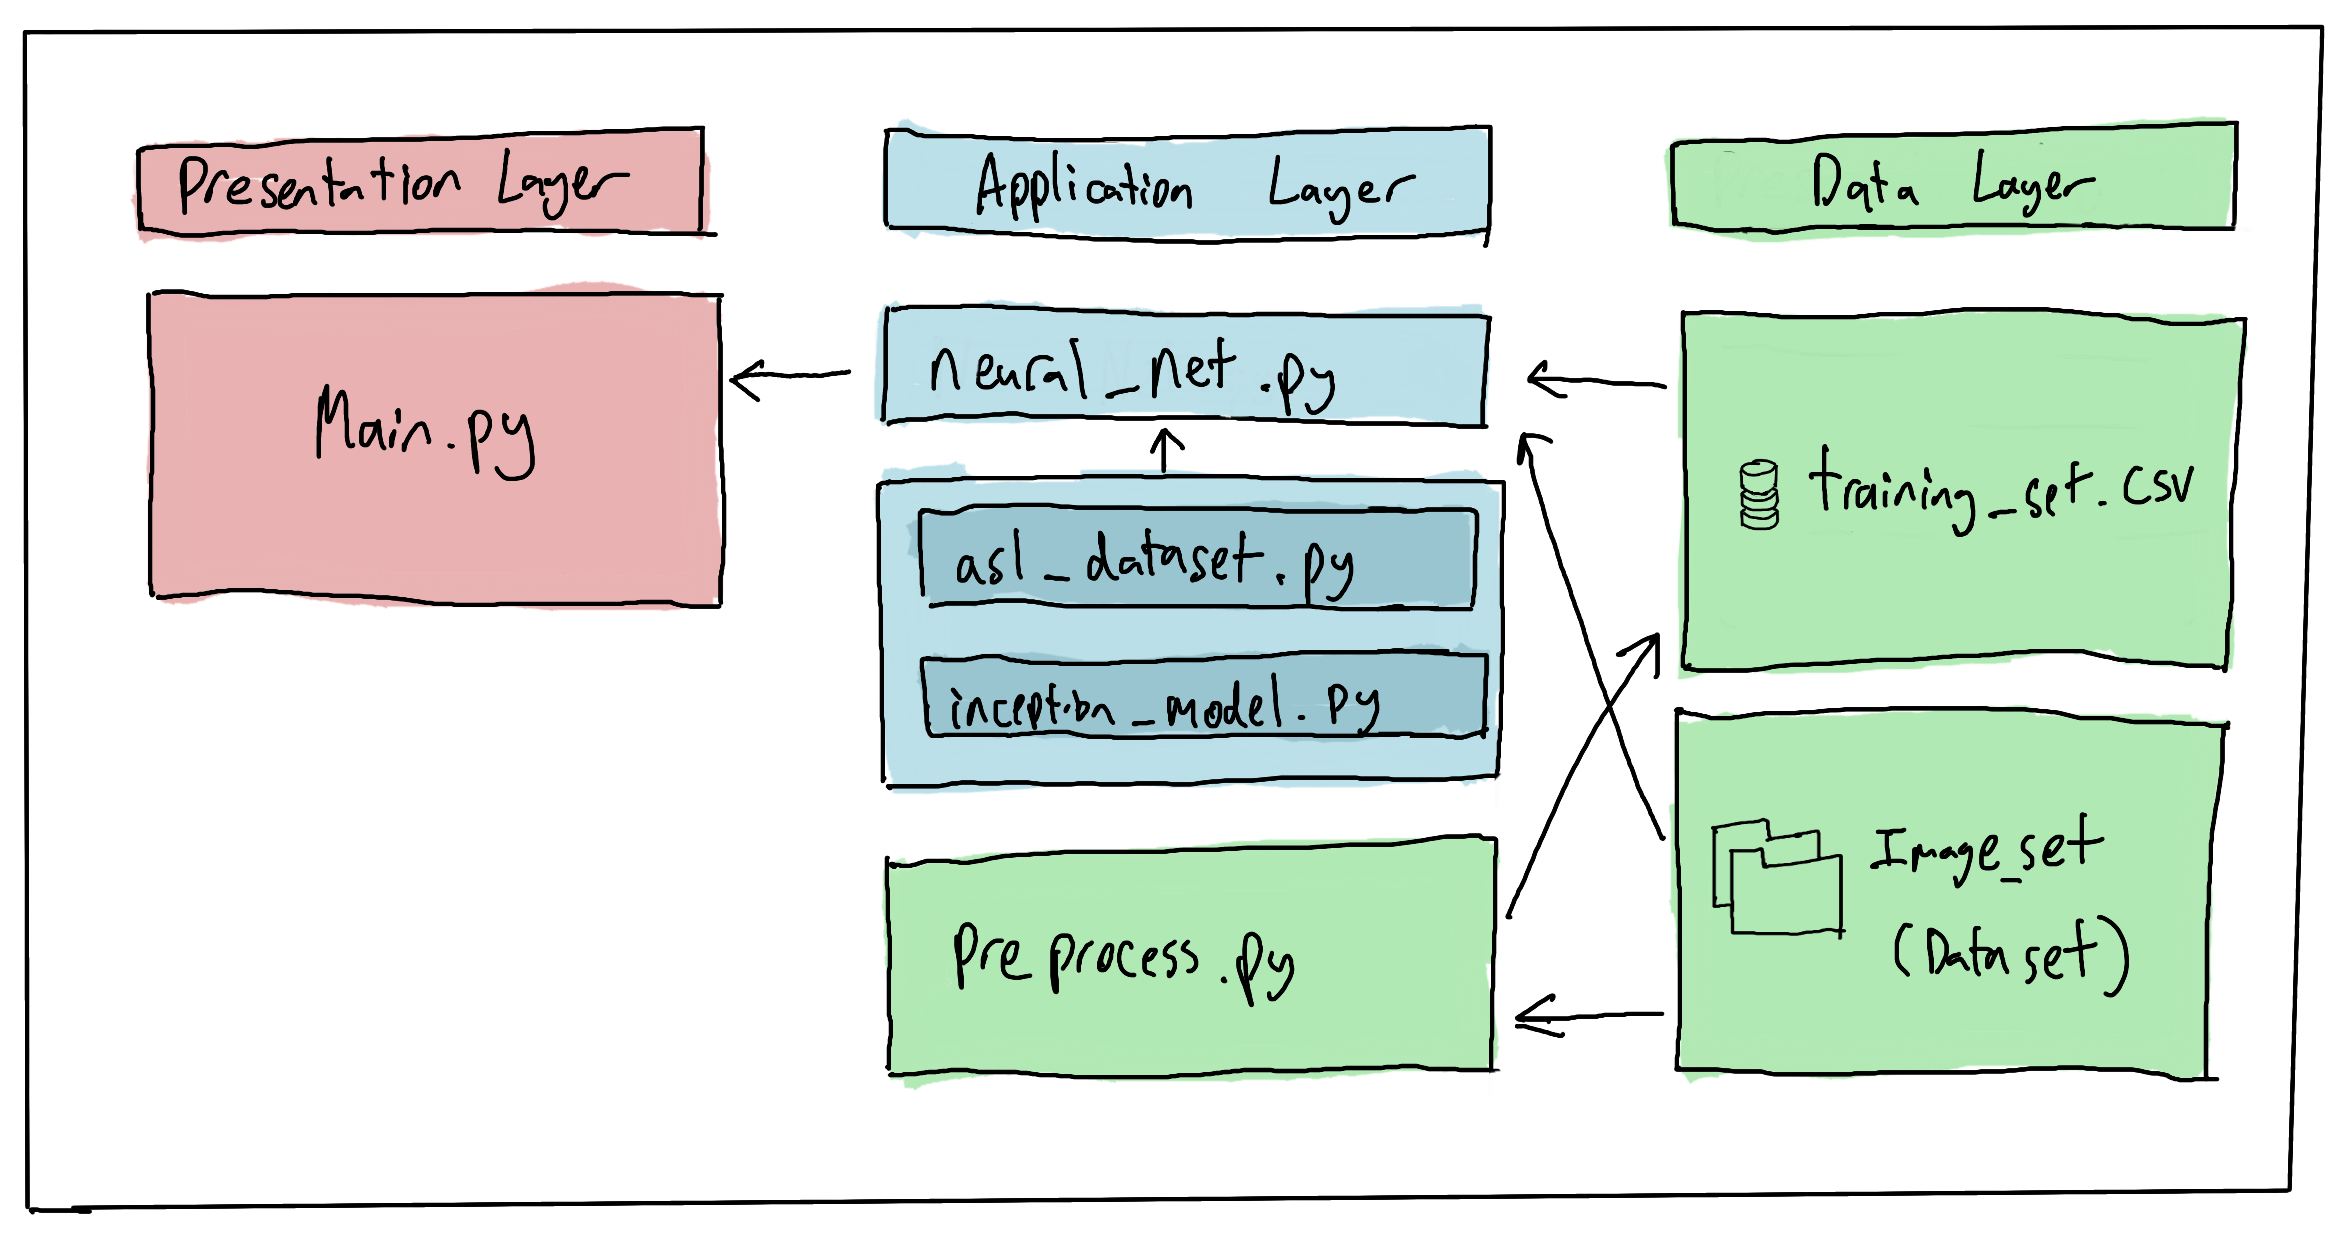
\includegraphics[width=13cm]{images/monolith1.png}
        \\
        \raggedright \textit{
        Figure 9: Visualisation of the interactions of each python modules within this monolithic system.
        }
    \end{center}

    This monolithic structure has 3 main layers - the presentation, application and data layer. The presentation layer is the module responsible for creating an intuitive interface for the users using OpenCV. The application layer is responsible for all the data preprocessing and all auxiliary functionalities for the program. The data layer simply contains the datasets and annotations required for the programs to be trained or ran. 

        \subsubsection{Data Preprocessing}
    The dataset used for this project is an ASL alphabet image set collected from Kaggle.com. The dataset is a directory with nested sub-directory each containing images of their respective classes. This dataset contains around 220,000 entries. The first step is to flatten all the directories, the name of the sub-directory is appended to each image in the format of: `subdir\_imagename'. Then the subdir will be hashed as the label to the image as the label has to be an integer. Due to each directory having only a single character representing the respective image class, the hash function is a simple typecast ($hash(x) = int(x)$). The results will be a output file named `annotations.csv' containing 2 columns - image\_name and label.
        
        \subsubsection{Neural Network Implementation}
    As stated above the architecture for the convolutional neural network used for this project will be the GoogLeNet. GoogLeNet consists of 3 convolutional layers, 9 inception modules (each with 1x1, 1x1$\rightarrow$3x3, 1x1$\rightarrow$5x5 convolution kernels and a 3x3 max pool), and 2 auxiliary softmax modules.

    \begin{center}
        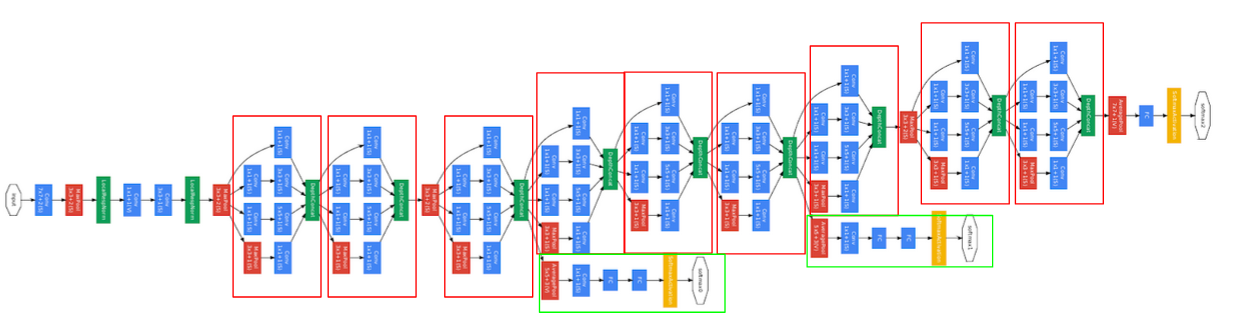
\includegraphics[width=16cm]{images/googlenet.png}
        \\
        \raggedright \textit{
        Figure 10: GoogLeNet architecture visualised. Red boxes are inception modules, green boxes are softmax modules.
        }
    \end{center}

    This is implemented with PyTorch in the neural\_network.py module. An auxiliary class in the asl\_dataset.py module, implemented with PyTorch, allows our model to get and read images based on an annotated csv. The custom ASL\_DATASET class overrides the `name-mangled' functions - \_\_init()\_\_, and \_\_getitem()\_\_. Before feeding the images into the neural network, each image will be downscaled to 255 by 255.

    Hyperparameters are as listed: max\_epoch = 32, learning\_rate = 0.00001, batch\_size = 256. Early stopping is implemented when the improvement in losses is less than 0.01 for more than 3 epochs. Batch size of 256 is as high as a 10GB VRAM GPU can handle. Loss function is naturally the cross entropy loss as this is a multi-class classification model, and the optimizer used is the adam optimizer. After every epoch, a checkpoint of the model's current weight and optimizer state will be saved. 

    \subsection{Dynamic Interpreter (Hand Landmark Approach)}
    This subsection will detail the overview of the implementation for the dynamic interface. This model is the \textbf{definitive} model for this project, and essentially renders the above model obselete (see comparative benchmarks in the evaluation section below). The modules explored in this section will include, the data preprocessing, hand landmarking, modular phonological trackers (symbols and movement), and all auxiliary functionalities. This will follow the monolithic structure shown in the diagram below:

    \begin{center}
        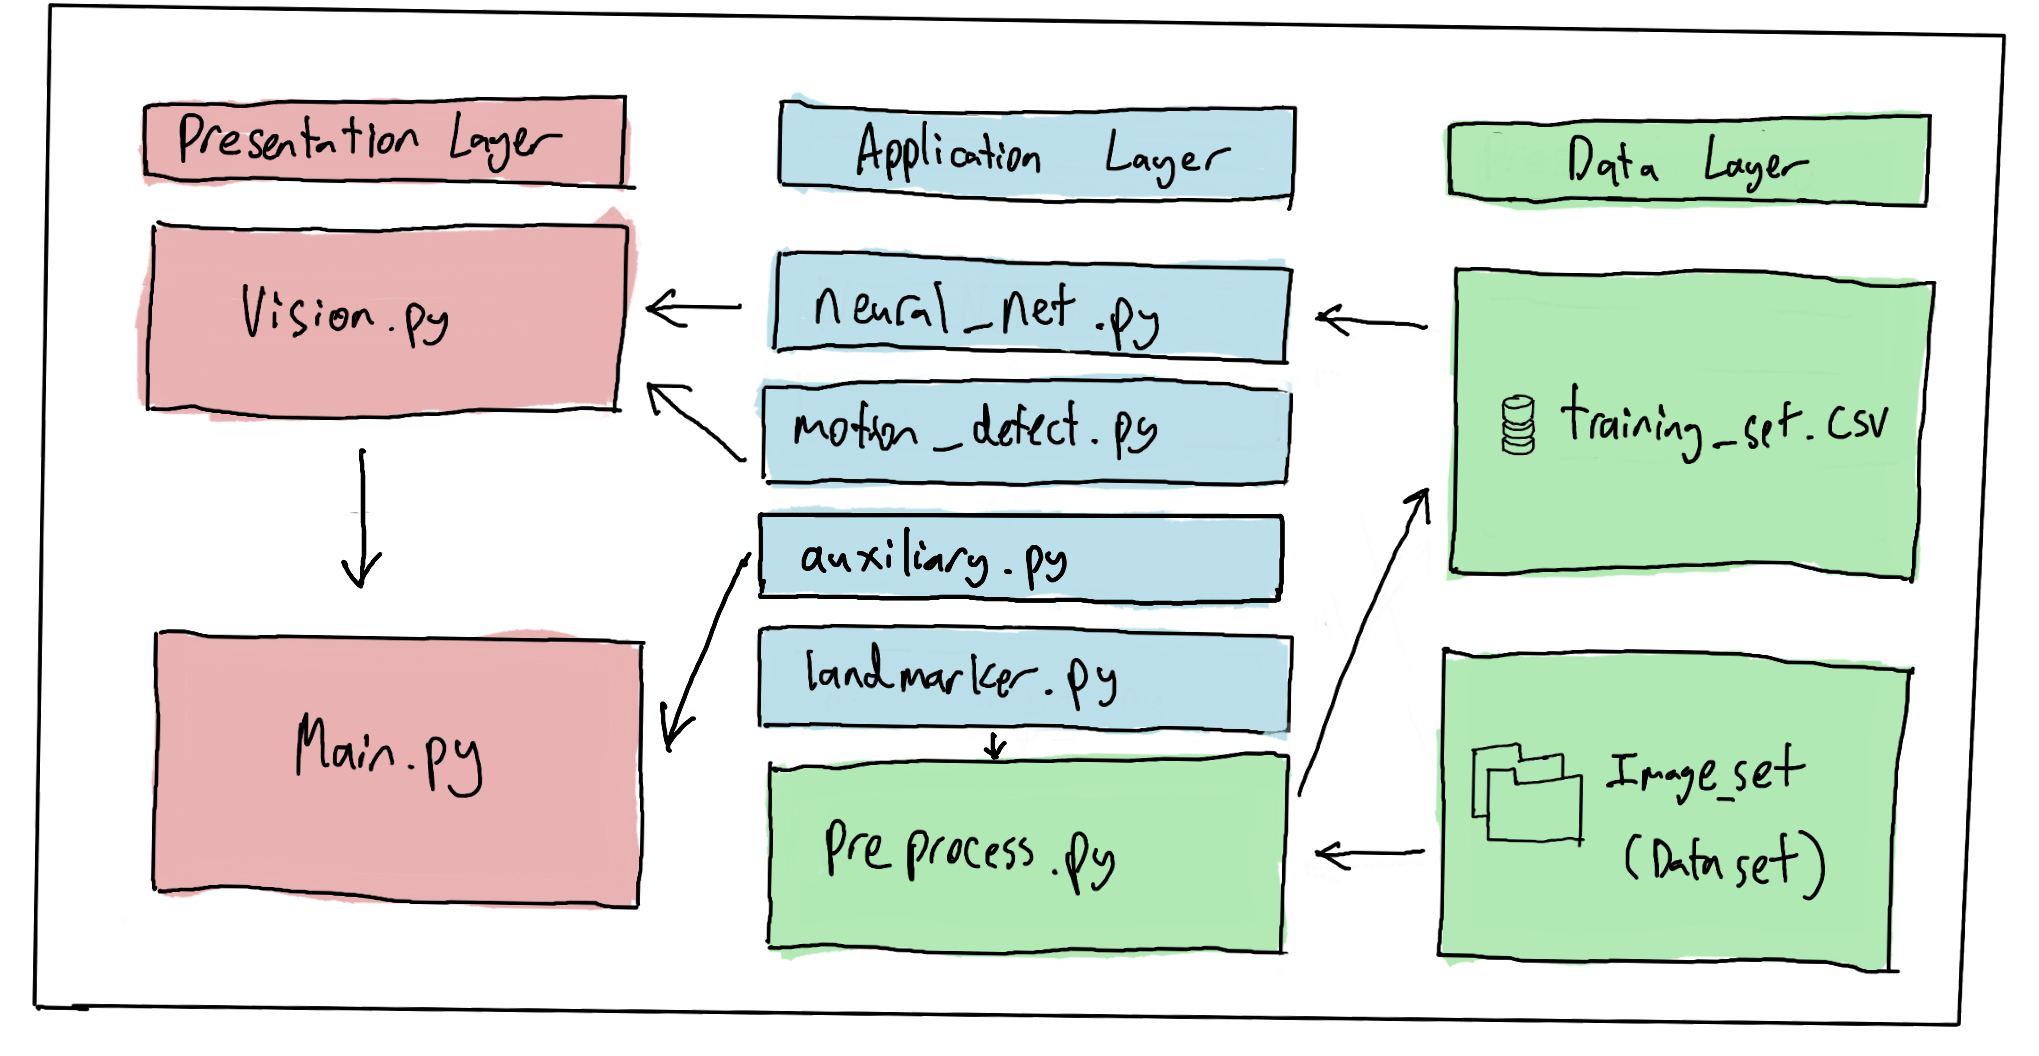
\includegraphics[width=13cm]{images/monolith2.png}
        \\
        \raggedright \textit{
        Figure 11: Visualisation of the interactions of each python modules within this monolithic system.
        }
    \end{center}

        \subsubsection{Hand Landmarking}
    The handlandmarking module had 2 iterations - OpenPose and MediaPipe. OpenPose is the bottom-up approach to pose estimation explored in the `pre-requisite knowledge' section above (see section 2.3). OpenPose while being a great option for the task had severe limitations. OpenPose is very difficult to implement given it is not a distributed framework but rather a model proposed in a research paper. OpenPose is also extremely hard to train. The model does not come with pre-trained weights and its training requires the multiview bootstrapping process. Multiview bootstrapping is a very difficult procedure to replicate in a non-lab scenario due to equipment requirements and camera syncing issues. There was an open-sourced implementation of OpenPose using PyTorchm, however, its weights were not nearly accurate enough for the needs of this project. The last problem with OpenPose was its speed. Every frame's inference will take around 160 GFLOPs, which is impossible for real-time inferences for CPU or mobile devices.
    
    Google's MediaPipe was chosen as the alternative used in the final iteration of the program. MediaPipe is a open-sourced library containing many pose estimation solutions and their pre-trained weights; however, MediaPipe is not without it's downsides. MediaPipe lacks any meaningful documentation other than demo codes. Using MediaPipe to the extent this project will need requires a deeper dive into the source code itself. MediaPipe is able to run at around 17ms (58 frames per second), on a mobile phone's CPU (Google Pixel 6) and around 12ms (83 frames per second), on the same phone's GPU.

    The landmarking module has 2 main functions - extracting landmarks, and rendering landmarks. Extracting landmarks is relatively simple as it simply takes in an image, processes it as a MediaPipe matrix then running the inference and returning the results. Rendering landmarks was especially tricky due to the complete lack of documentation regarding the formatting of the model's output. Rendering landmark was done using the help of OpenCV.

        \subsubsection{Data Preprocessing}
    The dataset used here is the same dataset collected from Kaggle from the subsection above. The main goal of the data preprocessing here is to match each image with label and every coordinate of every joints located within said image. There are 3 new main functions within this module - extracting landmarks and labelling csv from dataset, preprocessing csv, splitting annotations into testing and training sets. 
    
    \paraskip

    \noindent\textbf{Annotating Landmarks: } Dataset fed into this model has already been flattened using previous model's preprocessing module. First, labelling\_csv() creates a pandas dataframe containing 45 columns - image name, label, handedness (left or right), and 21 pairs of coordinates (x and y of landmarks). Each image is then iteratively feature extracted using the landmarking module, parsed, normalized and then mapped onto the dataframe. Normalisation process was explained in the architecture section above (section 4.3). 
    
    \paraskip

    \noindent\textbf{Preprocessing Annotations: } The second part of the module revolves around preprocessing the annotated data. There are 3 main tasks in this function - NaN purging, undersampling and changing label ranges. NaN purging is simply dropping all rows that contains NaN values. Sometimes the landmarker will forego a certain end joint if the finger or base of the palm extends beyond the screen; also, if the landmarker fails to detect a hand the coordinate columns for that row will also fill with NaNs. Undersampling is the process of removing random rows within certain groups to balance the amount of rows each group occupies. This is done to remove imbalance and prevent our neural network from skewing to the more prevalent class. This will result in data loss but it is negligable as post undersampling still results in around 110,000 total entries. Lastly, changing data range is simply compressing the hash established earlier. For example, integer casting the character `A' will result in 65 which will be labeled as 0 since its the smallest number in the label set (B is 1 instead of 66, so on so forth).

    The last part of the module simply splits the annotations into a training and testing set by a ratio of 10 to 1 respectively. There are also auxiliary functions, most notably to fetch additional information for data analysis like showing class distributions, etc.

        \subsubsection{Neural Network Implementation}
    The neural network used for this model is a vanilla MLP. It consists of 6 hidden layers (input > 128 > 256 > 316 > 512 > 256 > 128 > output), a single dropout layers (5\% total drop). Activation function used is the rectified linear unit function (ReLU). 

    \begin{center}
        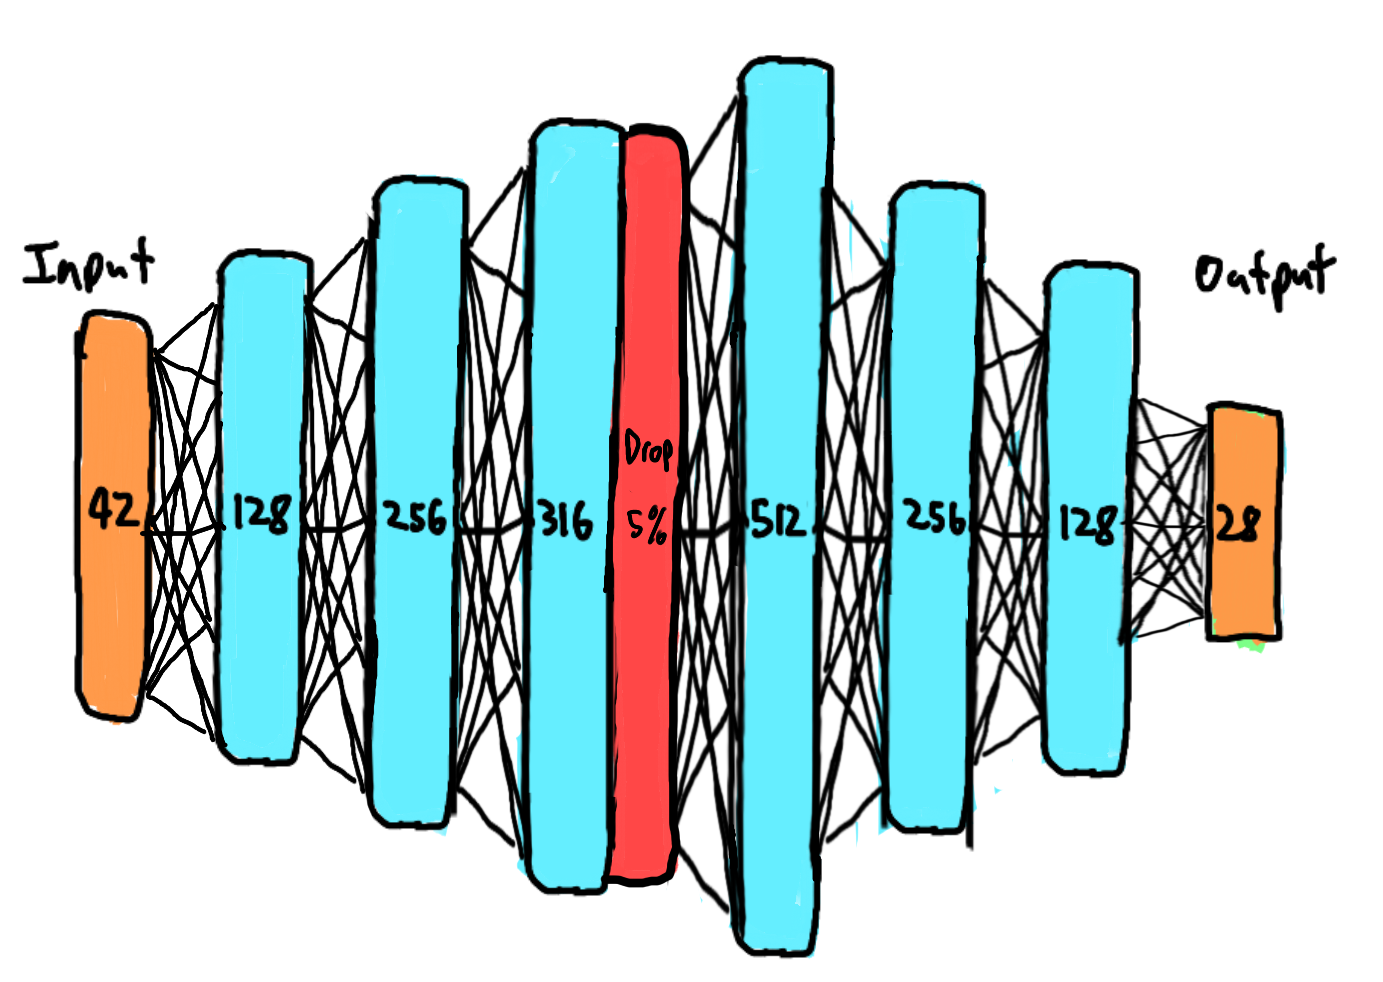
\includegraphics[width=8cm]{images/mlp.png}
        \\
        \raggedright \textit{
        Figure 12. Visualisation of the MLP used for the hand classification.
        }
    \end{center}

    This is implemented with PyTorch in the neural\_net.py module. This module includes a custom class representing the MLP and all its internal functions. All the required functions to feed forward, backpropagate, training, testing, and saving models and checkpoints are methods within the MLP class. For training the actual outputs have to be one-hot encoded as the output is the likelyhood of each class' prediction. One-hot encoding is a function used to map a group of labels into a table of possible labels; each column symbolizing whether or not the intial label is the current column's label. 

    Hyperparameters are as listed: max\_epoch = 900, learning\_rate = 0.0005. Early stopping is not implemented. Loss function is cross entropy loss for the same reason explained in the section above (see section 5.2.2). After every 50 epochs, a checkpoint of the model's current weights will be saved. 

    \subsection{Interface Implementation}
    The interfaces are contained within the vision.py module. The vision module implements various streaming interfaces using a video camera initialized via OpenCV. The camera allows us to use the video stream's individual frames for symbol classification, and even cross frame processing for motion detection and buffering. There are many streaming interfaces within this module; the one used for our final application is stream\_translation\_interface. 

    \paraskip
    \noindent\textbf{Main Interface: } This purpose of this interface is to output a full array of text based on tokens (previously defined in section 4.4). On every frame a symbol prediction will be made and will be logged into an buffering array, this buffering array will be used to make a true prediction. The buffering array works as a FIFO queue; if the queue is currently full, the latest prediction will enter the queue as the earliest prediction will exit. A true prediction is made on every frame based on the most frequent prediction within the prediction buffer. True prediction and true motion will be used as terms descibing the actual prediction and motions returned from the interface as tokens. The direction will be tracked using the method stated in section 4.3. After each frame's direction is calculated, it will, like symbol predictions, enter a buffering array. This motion buffer array will be used to calculate the true motion of the hand by logging every direction that composes more than 30\% of the whole buffer. The true motion, unlike true prediction, will only be calculated and logged as token when the true prediction changes. The output of this particular interface will be a sentence made out of tokens, formatted like: $sentence = [token]$, $token = [symbol, [directions]]$.

    \paraskip
    \noindent\textbf{Other Interfaces: } There are other intefaces within this module as well. For example, there is an I/O interface for typing by signing letters, a benchmarking interface for symbol inference speed analysis, et cetera. As useful as these interfaces are, it is important to note none of these interfaces are used in the final application for this project.


\section{Evaluation and Approach Comparison}
    \subsection{Evaluation Methodations}
        Evaluation will consist of 2 main parts - speed and accuracy. Considering the goal of this project is a proof of concept for a \textbf{real-time} visual-manual interface, speed is equally if not more important than accuracy. Accuracy is measured through running each model through a specific dataset that is designed to push the model's accuracy to its limits. This testing dataset will feature a variety of different ambient lighting, degrees of motion blur, background and hand sizes (distance from camera). 

        \paraskip

        \noindent\textbf{Accuracy Analysis: } Accuracy will be measured by a variety of factors - the confusion matrix, recall scores, precision scores and most importantly the F1 score. The confusion matrix is a table of values filled with the frequency of predictions. This confusion matrix has 2 axis - the true classes and the predicted classes, each class then has it's class specific matrix. The class specific matrix is split into 4 categories - True Positive (TP), False Positive (FN), True Negative (TN), and False Negative (FN). The TN is when both the prediction and the true class aligns; FP is when the specified class is predicted but does not align with the true class; TN is when the non-true classes are not predicted; FN is when the prediction does not align with the true class.

        \begin{center}
            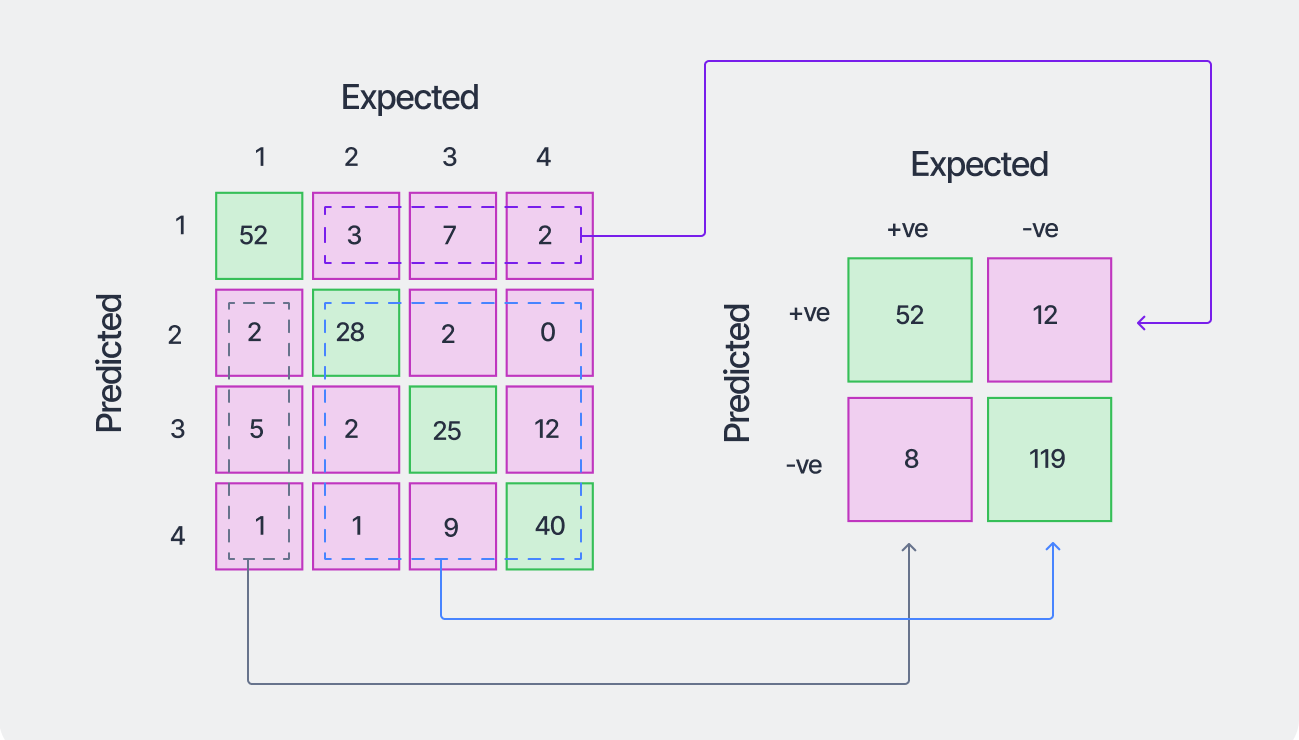
\includegraphics[width=9cm]{images/confusionclass.png}
            \\
            \raggedright \textit{
            Figure 6: Visual representation of how to convert a multi-class confusion matrix into a class specific confusion matrix.
            }
        \end{center}

        We can then calculate it's precision and recall score based on the class-specific confusion matrix we have extracted. Since, there will be a precision and recall score per class, the evaluation will offer the chance to monitor both the metrics of specific hard to classify classes and the mean metrics of the model. The precision score is the number of correct predictions out of all the predicted positive predictions. The recall score is the number of correct predictions out of all the true prredictions. The F1 score would simply be a harmonic mean of both the prediction and recall scores, also the main metric to be used to judge the model's efficacy. The equations to calculate these metrics is as follows:

        \vskip 0.3cm
        \[Precision = \frac{TP}{TP+FP} \qquad{}
        Recall = \frac{TP}{TP+FN} \qquad{}
        F1 = 2*\frac{Precision * Recall}{Precision + Recall}\]
        \vskip 0.3cm
        

        \noindent\textbf{Speed Analysis: } Speed is measured by 2 main factors - process speed per frame and scalability. Process speed per frame is measured in milliseconds and is the average speed of which the model takes to classify a single hand pose. The lower the process speed, the higher the frames processed per second, and the more viable the model is for real-time applications. Scalability is equally as important as practical speed. This metric shows how many more milliseconds the model will add to its process speed per frame when a new class is added to the model. The lower the additional milliseconds it takes to learn to identify a new class the more scalable this model will be to actual applications (potentially hundred of classes needed). The main metric to be used to judge the model's speed is the mean millisecond per frame of the entire testset.

    \subsection{Testing Set}
        A testing set that is completely disjoint from the original dataset will have to be collected. This is due to the images from the original dataset being too similar to each other. This led to the initial round of testing on a subsection of the original dataset having an accuracy score that does not reflect the true performance of the models. 

        \paraskip

        \noindent\textbf{Collecting Testing Set: } The testing set will be collected using a python script - data\_collect.py. This script contains 2 functions - collect\_symbol, and collect\_dataset. The collect\_symbol function takes in 4 arguments: symbol\_name, which is a string that the file saved will be named after (e.g. if symbol name is "A", the saved images will be named [A\_1, A\_2, A\_3...]); max\_collect, which determines how many images to collect in total; segments, which determines how many pauses for user input the script will make in the middle of collection; and lastly, throttle\_limit, which is the amount of seconds it will take for the stream to capture a frame for the dataset. The collect\_symbol function collects the an arbitrary number of samples by starting a video stream using OpenCV, after every `throttle\_limit' worth of time passes an image will be saved and writtent to the dataset. When $current\_collected$ \% $ (max\_collect/segments) = 0$, the script will pause and wait for user input until continuing collection. This is to allow for a change in background, lighting or anything that can add more variance to the dataset. The formula above is to split the amount to collect into equal segments to pause on.
        
        \paraskip

        \noindent\textbf{Collected Testing Set: } The resulting dataset collected for testing includes 40 different images per the 25 symbols, (1000 in total). The letter "Z" is excluded from the model due to its nature of being classified based on motion. The testing set is also preprocessed using the methods stated above (see section 5.2.1 and 5.3.2) to obtain it's individual csv annotations for testing.

    \subsection{Metrics}
        This subsection will show the accuracy, recall, precision and f1 scores per class, for each of the 2 models. From there, an aggregate macro f1, recall and precision will also be calculated and compared. Time for inference and time for training will also be shown. Respective hardware for the collection of the speed metrics will also be listed

        \paraskip

        \noindent\textbf{GoogLeNet Metrics (Accuracy): } 
        The overall accuracy of the model is 0.635 (635/1000 accurate inferences). The macro F1 score is 0.617. The macro precision score is 0.661. The macro recall score is 0.634.

        \begin{center}
            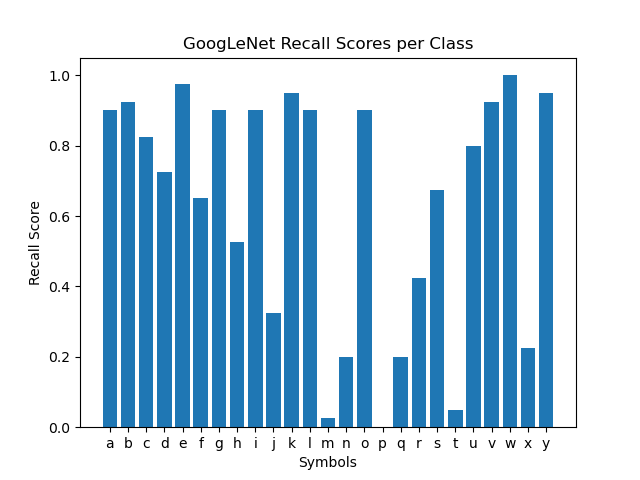
\includegraphics[width=8cm]{images/gnetrecall.png}
            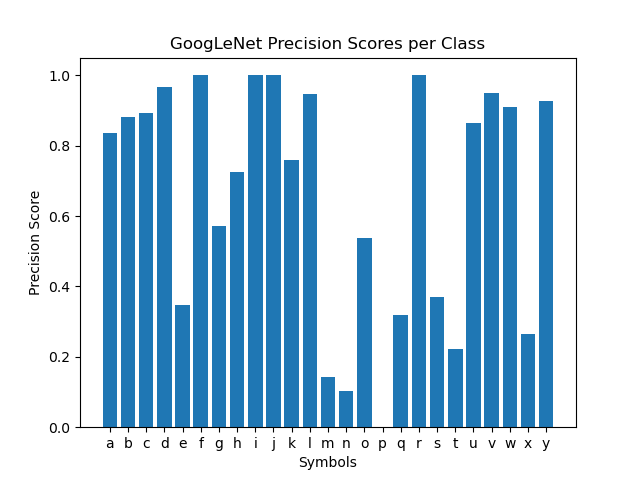
\includegraphics[width=8cm]{images/gnetprec.png}
            \\
            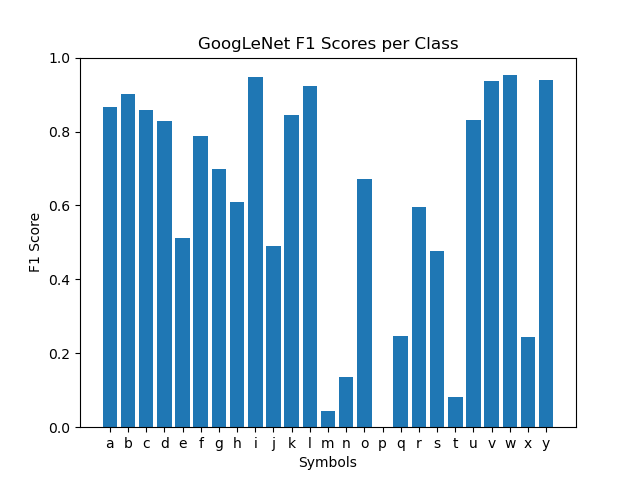
\includegraphics[width=8cm]{images/gnetf1.png}
            \\
            \raggedright \textit{
            Figure 12: GoogLeNet F1, Precision and Recall scores per class.
            }
        \end{center}

        \paraskip

        \noindent\textbf{GoogLeNet Metrics (Speed): }
        The time it took for this model to classify 1001 images was 43.694s (mean average of 43.65 ms per inference). Assuming no overhead to the application, this model will run real-time at around 23 frames per second. Inference is performed on CPU on the Apple M2 chip of a Macbook Pro.

        Training time for this model took around 52hrs before early stopping kicked in at epoch 14. Training is performed on 8704 CUDA cores on an Nvidia RTX3080 10GB VRAM GPU.

        \paraskip

        \noindent\textbf{Definitive Model Metrics (Accuracy): } 
        The overall accuracy of the model is 0.743 (743/1000 accurate inferences). The macro F1 score is 0.729. The macro precision score is 0.772. The macro recall score is 0.742.

        \begin{center}
            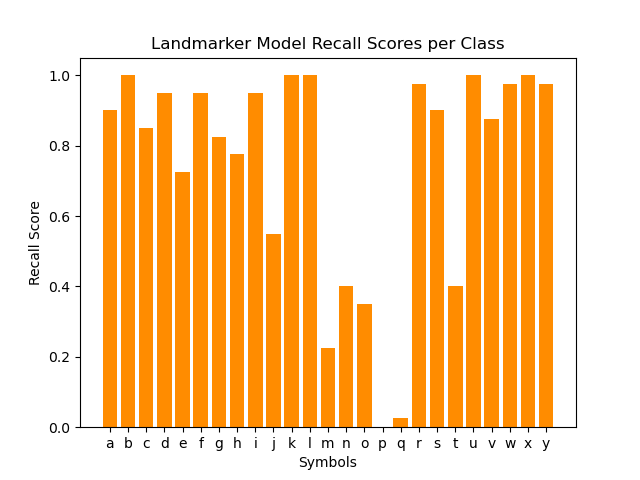
\includegraphics[width=8cm]{images/htrecall.png}
            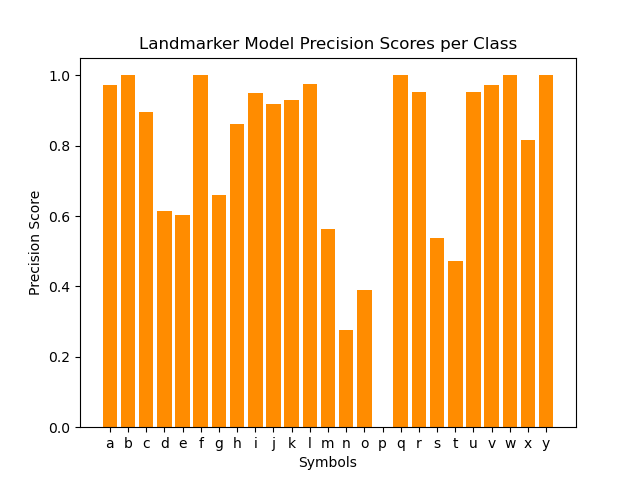
\includegraphics[width=8cm]{images/htprec.png}
            \\
            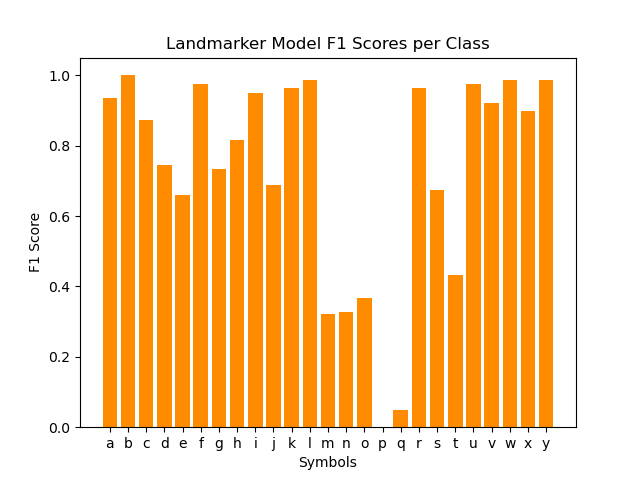
\includegraphics[width=8cm]{images/htf1.png}
            \\
            \raggedright \textit{
            Figure 13: My Model's F1, Precision and Recall scores per class.
            }
        \end{center}

        \noindent\textbf{Definitive Model Metrics (Speed): }
        The time it took for this model to classify 1001 images was 27.089s (mean average of 27.06 ms per inference). Assuming no overhead to the application, this model will run real-time at around 37 frames per second. Inference is performed on CPU on the Apple M2 chip of a Macbook Pro.

        Training time for this model took 27.28 seconds, training fully on all 900 epochs. Training is performed on 8704 CUDA cores on an Nvidia RTX3080 10GB VRAM GPU for consistency. Training for the handtracking module is not relevant (for scaling) as it has already been trained and never has to be trained again for any future application (constant time).

    \subsection{Analysis and Comparison}
        This subsection will analyse and compare each model and their accuracy and speed metrics. This section will also dissect and explore outliers and the potential reasoning behind them.

        \paraskip

        \noindent\textbf{Accuracy Metrics Per Class: } Here is a comparative bar chart of the F1 score between both models. This is the main metric used to evaulate the accuracy performance, the other accuracy metrics will also be explored for their own reasons. To better understand this section, it is recommended to review the ASL letters to learn how each symbol looks.

        \begin{center}
            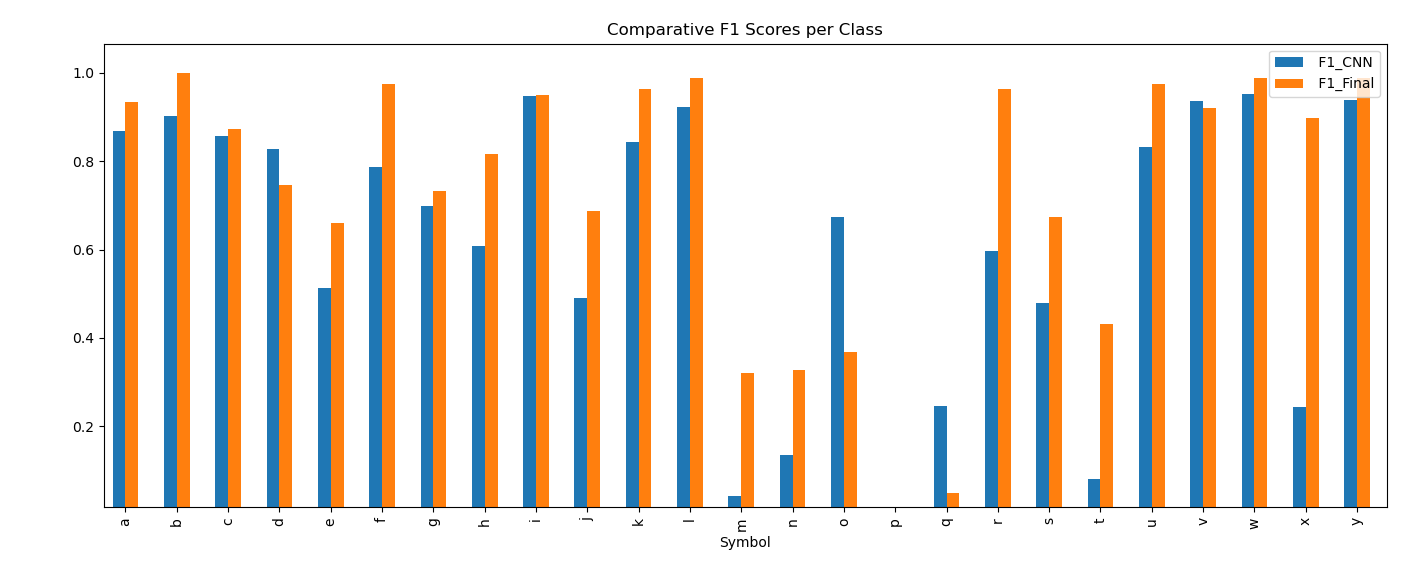
\includegraphics[width=16cm]{images/f1compare.png}
            \\
            \raggedright \textit{
            Figure 14: Comparison of F1 Scores across both models (`F1\_CNN' is GoogLeNet, `F1\_Final' is custom model).
            }
        \end{center}

        The consistancy of F1 in our model is drastically better than GoogLeNet's. The F1 scores are also generally higher across the board other than the letters `O' and `Q'. Upon further inspection, our custom model often confuses the letter `O' and `C' depending on where the closed loop points. This explains the high recall but low precision on the letter `C' Our custom model also struggles with hand poses where the palm is pointed downwards, leading to very inaccurate `P' and `Q' predictions. However, when the model does infer a `Q' prediction, it is always correct (1.0 precision on `Q'). These problems can be alleviated with higher quality training data and even an additional parameter to the neural network (palm orientation). It is important to note, on the real time applications where temporal information is available, the letter `O' is classified very consistantly. Both models struggle with poses that are formed with closed fists (`T', `M', `N'). The reason for this is because these symbols are oftentimes mistaken as `S', hence the recall being significantly higher than the precision for this symbol in both models. The last outlier is `P' for some reason both model refuses to classify the letter `P'. After investigation, it is found that the letter `P' used in the training dataset collected from Kaggle is inconsistant from the `P' commonly used in ASL. If we disregard this outlier, the each macro metrics will be increased by 4.17\% (25/24) per model.

        \paraskip

        \noindent\textbf{Metric Comparison: } Discounting the difficult signs, the overall stability of F1 over all classes is significantly higher on the landmark assisted model. The improvement in macro F1, recall, and precision scores in the landmarker model compared to GoogLeNet is approximately 18.15\%, 16.79\%, and 17.03\% respective. Overall accuracy improvement is at 17.01\%. This is a very noticeable improvement on the real-time application. 

        Now onto the speed metrics, which is the main determining factor of scalability and real-time uses. The training time for each model is incomparbly large; there is around a 693333\% improvement between 52 hours (GoogLeNet) vs 27 seconds (My model). It is HIGHLY infeasible to continuously retrain GoogLeNet to add new symbol and features compared to my model. The inference time per frame is also a substantial improvement from GoogLeNet to my model, there is a 37.5\% increase in speed.

\section{Conclusion}
    \subsection{Critical Analysis of Limitations}
    There are 2 main types of limitations to this project - developmental limitations, and feature limitations. Developmental limitations are the limitations imposed during development of the project, and feature limitations are potential unimplemented features (additional scope) that because of time and resource restraint has not been achieved in this project.

    \paraskip

    \noindent\textbf{Developmental Limitations: } The major noticeable limitation to development is the poor quality training data. The dataset collected from Kaggle (which was the best one available), had many images that were functionally duplicates of each other. Within every class there will be groups of images with virtually no deviance between them. There is also a problem with certain classes having the hands shot from a single angle making inferences less accurate in more complex poses. Another limitation is the fact that every hand pose is classified into a category. This can be mediated by implementing an lower limit to the output score; if no classes have an output score above the limit it should classify as `unknown'.

    \paraskip

    \noindent\textbf{Feature Limitations: } There are a few main unimplemented features that could be implemented to improve ASL translation. The translation process could be replaced from an explicit one to a deep learning one. A palm orientation tracker could could allow for more diverse movement (such as palm rotations) and more accurate classification (through rotational normalisation). Scaling to other phonological parameters with technologies such as a one-look hand + facial landmarking model. The possibilities are endless but realistically those would be the first steps to take towards a better ASL translator.

    \subsection{Conclude}
    The applications of a visual manual interface is limitless, we could create educational tools for signed languages through gamification, we could create futuristic I/O devices for virtual reality. A fully documented open sourced version of the application will be hosted on my GitHub. This will hopefully allow for future research and innovations built upon OpenHandmark to improve the livelyhoods of people.


\pagebreak 

\begin{thebibliography}{30}
    \bibitem{greedy2} Programiz, \emph{"Greedy Algorithm"}, Available at: \url{https://www.programiz.com/dsa/greedy-algorithm}

    \bibitem{boruvka} O. Boruvka, \emph{"O jistém problému minimálním - About a certain minimal problem"}, Práce Mor. Přírodověd. Spol. V Brně III, 1926

    \bibitem{lemma} H. Nicholas, \emph{"Handbook of Writing for the Mathematical Sciences"}, Society for Industrial and Applied Mathematics, pp. 16, 1998.

    \bibitem{waterloo lemma} R. Oliveira, \emph{"Lecture 13: Minimum Spanning Trees"}, University of Waterloo Cheriton School of Computer Science, 2023, Accessed at: \url{https://student.cs.uwaterloo.ca/~cs341/lectures/lecture13.pdf}

    \bibitem{union find} R. E. Tarjan, \emph{"Efficiency of a Good But Not Linear Set Union Algorithm"}, Journal of the ACM, 1975
    
    \bibitem{chazelle} B. Chazelle, \emph{"A minimum spanning tree algorithm with inverse-Ackermann type complexity"}, J. ACM, 2000 

\end{thebibliography}


\end{document}
